\documentclass{article}
\usepackage{ifluatex}
\ifluatex 
    \usepackage{fontspec}
    \setsansfont{CMU Sans Serif}%{Arial}
    \setmainfont{CMU Serif}%{Times New Roman}
    \setmonofont{CMU Typewriter Text}%{Consolas}
    \defaultfontfeatures{Ligatures={TeX}}
\else
    \usepackage[T2A]{fontenc}
    \usepackage[utf8]{inputenc}
\fi
\usepackage[english,russian]{babel}
\usepackage{amssymb,latexsym,amsmath,amscd,mathtools,wasysym}
\usepackage[shortlabels]{enumitem}
\usepackage[makeroom]{cancel}
\usepackage{graphicx}
\usepackage{geometry}
\usepackage{verbatim}
\usepackage{fvextra}

\usepackage{longtable}
\usepackage{multirow}
\usepackage{multicol}
\usepackage{tabu}
\usepackage{arydshln} % \hdashline and :

\usepackage{float}
\makeatletter
\g@addto@macro\@floatboxreset\centering
\makeatother
\usepackage{caption}
\usepackage{csquotes}
\usepackage[bb=dsserif]{mathalpha}
\usepackage[normalem]{ulem}

\usepackage[e]{esvect}
\let\vec\vv

\usepackage{xcolor}
\colorlet{darkgreen}{black!25!blue!50!green}


%% Here f*cking with mathabx
\DeclareFontFamily{U}{matha}{\hyphenchar\font45}
\DeclareFontShape{U}{matha}{m}{n}{
    <5> <6> <7> <8> <9> <10> gen * matha
    <10.95> matha10 <12> <14.4> <17.28> <20.74> <24.88> matha12
}{}
\DeclareSymbolFont{matha}{U}{matha}{m}{n}
\DeclareFontFamily{U}{mathb}{\hyphenchar\font45}
\DeclareFontShape{U}{mathb}{m}{n}{
    <5> <6> <7> <8> <9> <10> gen * mathb
    <10.95> matha10 <12> <14.4> <17.28> <20.74> <24.88> mathb12
}{}
\DeclareSymbolFont{mathb}{U}{mathb}{m}{n}

\DeclareMathSymbol{\defeq}{\mathrel}{mathb}{"15}
\DeclareMathSymbol{\eqdef}{\mathrel}{mathb}{"16}


\usepackage{trimclip}
\DeclareMathOperator{\updownarrows}{\clipbox{0pt 0pt 4.175pt 0pt}{$\upuparrows$}\hspace{-.825px}\clipbox{0pt 0pt 4.175pt 0pt}{$\downdownarrows$}}
\DeclareMathOperator{\downuparrows}{\clipbox{0pt 0pt 4.175pt 0pt}{$\downdownarrows$}\hspace{-.825px}\clipbox{0pt 0pt 4.175pt 0pt}{$\upuparrows$}}

\makeatletter
\providecommand*\deletecounter[1]{%
    \expandafter\let\csname c@#1\endcsname\@undefined}
\makeatother


\usepackage{hyperref}
\hypersetup{
    %hidelinks,
    colorlinks=true,
    linkcolor=darkgreen,
    urlcolor=blue,
    breaklinks=true,
}

\usepackage{pgf}
\usepackage{pgfplots}
\pgfplotsset{compat=newest}
\usepackage{tikz,tikz-3dplot}
\usepackage{tkz-euclide}
\usetikzlibrary{calc,automata,patterns,angles,quotes,backgrounds,shapes.geometric,trees,positioning,decorations.pathreplacing}
\pgfkeys{/pgf/plot/gnuplot call={T: && cd TeX && gnuplot}}
\usepgfplotslibrary{fillbetween,polar}
\ifluatex
\usetikzlibrary{graphs,graphs.standard,graphdrawing,quotes,babel}
\usegdlibrary{layered,trees,circular,force}
\else
\errmessage{Run with LuaTeX, if you want to use gdlibraries}
\fi
\makeatletter
\newcommand\currentnode{\the\tikz@lastxsaved,\the\tikz@lastysaved}
\makeatother

%\usepgfplotslibrary{external} 
%\tikzexternalize

\makeatletter
\newcommand*\circled[2][1.0]{\tikz[baseline=(char.base)]{
        \node[shape=circle, draw, inner sep=2pt,
        minimum height={\f@size*#1},] (char) {#2};}}
\makeatother

\newcommand{\existence}{{\circled{$\exists$}}}
\newcommand{\uniqueness}{{\circled{$\hspace{0.5px}!$}}}
\newcommand{\rightimp}{{\circled{$\Rightarrow$}}}
\newcommand{\leftimp}{{\circled{$\Leftarrow$}}}

\DeclareMathOperator{\sign}{sign}
\DeclareMathOperator{\Cl}{Cl}
\DeclareMathOperator{\proj}{pr}
\DeclareMathOperator{\Arg}{Arg}
\DeclareMathOperator{\supp}{supp}
\DeclareMathOperator{\diag}{diag}
\DeclareMathOperator{\tr}{tr}
\DeclareMathOperator{\rank}{rank}
\DeclareMathOperator{\Lat}{Lat}
\DeclareMathOperator{\Lin}{Lin}
\DeclareMathOperator{\Ln}{Ln}
\DeclareMathOperator{\Orbit}{Orbit}
\DeclareMathOperator{\St}{St}
\DeclareMathOperator{\Seq}{Seq}
\DeclareMathOperator{\PSet}{PSet}
\DeclareMathOperator{\MSet}{MSet}
\DeclareMathOperator{\Cyc}{Cyc}
\DeclareMathOperator{\Hom}{Hom}
\DeclareMathOperator{\End}{End}
\DeclareMathOperator{\Aut}{Aut}
\DeclareMathOperator{\Ker}{Ker}
\DeclareMathOperator{\Def}{def}
\DeclareMathOperator{\Alt}{Alt}
\DeclareMathOperator{\Sim}{Sim}
\DeclareMathOperator{\Int}{Int}
\DeclareMathOperator{\grad}{grad}
\DeclareMathOperator{\sech}{sech}
\DeclareMathOperator{\csch}{csch}
\DeclareMathOperator{\asin}{\sin^{-1}}
\DeclareMathOperator{\acos}{\cos^{-1}}
\DeclareMathOperator{\atan}{\tan^{-1}}
\DeclareMathOperator{\acot}{\cot^{-1}}
\DeclareMathOperator{\asec}{\sec^{-1}}
\DeclareMathOperator{\acsc}{\csc^{-1}}
\DeclareMathOperator{\asinh}{\sinh^{-1}}
\DeclareMathOperator{\acosh}{\cosh^{-1}}
\DeclareMathOperator{\atanh}{\tanh^{-1}}
\DeclareMathOperator{\acoth}{\coth^{-1}}
\DeclareMathOperator{\asech}{\sech^{-1}}
\DeclareMathOperator{\acsch}{\csch^{-1}}

\newcommand*{\scriptA}{{\mathcal{A}}}
\newcommand*{\scriptB}{{\mathcal{B}}}
\newcommand*{\scriptC}{{\mathcal{C}}}
\newcommand*{\scriptD}{{\mathcal{D}}}
\newcommand*{\scriptF}{{\mathcal{F}}}
\newcommand*{\scriptH}{{\mathcal{H}}}
\newcommand*{\scriptK}{{\mathcal{K}}}
\newcommand*{\scriptL}{{\mathcal{L}}}
\newcommand*{\scriptM}{{\mathcal{M}}}
\newcommand*{\scriptP}{{\mathcal{P}}}
\newcommand*{\scriptQ}{{\mathcal{Q}}}
\newcommand*{\scriptR}{{\mathcal{R}}}
\newcommand*{\scriptT}{{\mathcal{T}}}
\newcommand*{\scriptU}{{\mathcal{U}}}
\newcommand*{\scriptX}{{\mathcal{X}}}
\newcommand*{\Cnk}[2]{\left(\begin{matrix}#1\\#2\end{matrix}\right)}
\newcommand*{\im}{{\mathbf i}}
\newcommand*{\id}{{\mathrm{id}}}
\newcommand*{\compl}{^\complement}
\newcommand*{\dotprod}[2]{{\left\langle{#1},{#2}\right\rangle}}
\newcommand\matr[1]{\left(\begin{matrix}#1\end{matrix}\right)}
\newcommand\matrd[1]{\left|\begin{matrix}#1\end{matrix}\right|}
\newcommand\arr[2]{\left(\begin{array}{#1}#2\end{array}\right)}

\DeclareMathOperator{\divby}{\scalebox{1}[.65]{\vdots}}
\DeclareMathOperator{\toto}{\rightrightarrows}
\DeclareMathOperator{\ntoto}{\not\rightrightarrows}

\newcommand{\undercolorblack}[2]{{\color{#1}\underline{\color{black}#2}}}
\newcommand{\undercolor}[2]{{\colorlet{tmp}{.}\color{#1}\underline{\color{tmp}#2}}}

\usepackage{adjustbox}

\geometry{margin=1in}
\usepackage{fancyhdr}
\pagestyle{fancy}
\fancyfoot[L]{}
\fancyfoot[C]{Иванов Тимофей}
\fancyfoot[R]{\pagename\ \thepage}
\fancyhead[L]{}
\fancyhead[R]{\leftmark}
\renewcommand{\sectionmark}[1]{\markboth{#1}{}}

\setcounter{tocdepth}{5}
\usepackage{amsthm}
\usepackage{chngcntr}

\theoremstyle{definition}
\newtheorem{definition}{Определение}
\counterwithin*{definition}{section}

\theoremstyle{plain}
\newtheorem{theorem}{Теорема}
\counterwithin*{theorem}{section} % Without changing appearance
\newtheorem{lemma}{Лемма}
\counterwithin*{lemma}{section}
\newtheorem{corollary}{Следствие}[theorem]
\counterwithin{corollary}{theorem} % Changing appearance
\counterwithin{corollary}{lemma}
\newtheorem*{claim}{Утверждение}
\newtheorem{property}{Свойство}[definition]

\theoremstyle{remark}
\newtheorem*{remark}{Замечание}
\newtheorem*{example}{Пример}


%\renewcommand\qedsymbol{$\blacksquare$}

\counterwithin{equation}{section}


\usepackage[outputdir=T:/TeX, cachedir=_minted-caches]{minted}
\usemintedstyle{tango}

\usepackage{calc}
\usepackage{forest}

\makeatletter
\renewcommand*{\minted@cleancache}{}
\makeatother

\fancyhead[L]{Операционные системы (базовый курс)}

\begin{document}
    \tableofcontents\pagebreak
    \section{Зачем нужна операционная система.}
    Что такое вычислительный узел на базовом уровне? У нас есть какое-то железо (процессоры, оперативка, кэши, различные другие штуки), у нас есть ПО, и есть пользователь. Если у нас есть одна программа и 1 пользователь, ОС была бы не нужна. Потому что ОС распределяет ресурсы между программами, защищает одну программу от ошибок другой и т.д.
    
    Но как только программ много, появляется конкуренция. Понятно, что нас не устраивает ситуация, когда побеждает сильнейший. Поэтому появляются какие-то правила, как надо жить. Как у нас в социологии сначала были традиции, их потом поддерживала религия, а потом составляли кодексы, так ситуация состоит и с программами. Но выполнение всех правил надо контролировать. Что сделали люди? Создали государство. Аналогично тут мы создаём набор программного обеспечения и наделяем его монополией на власть и насилие.
    
    А потом у нас получается несколько пользователей: сущностей более развитых, чем любая программа, и периодически желающих обойти закон. Поэтому теперь нам надо создать слой абстракции, не позволяющей пользователю напрямую управлять чем-либо.
    
    Этот слой абстракции~--- это ОС. Именно для этого она в первом приближении нужна.
    \begin{definition}
        \textbf{Операционная система}~--- базовое системное программное обеспечение, управляющее работой вычислительного узла и реализующее универсальный интерфейс между аппаратным обеспечением, программным обеспечением и пользователем.
    \end{definition}
    Что всё это значит? <<Базовое>>~--- нельзя без него, <<системное>>~--- не приносящее пользу напрямую.
    \begin{figure}[H]
        \begin{tikzpicture}
            \node[draw, ellipse] (OS) at (0,0) {OS};
            \node[draw, ellipse, below=of OS] (Hard) {Hardware};
            \node[draw, ellipse, above=of OS] (Soft) {Software};
            \node[draw, ellipse, right=of OS] (Users) {Users};
            \draw[->] ($(OS.north)!.33!(OS.north east)$) -- (\currentnode |- Soft.south);
            \draw[<-] ($(OS.north)!.33!(OS.north west)$) -- (\currentnode |- Soft.south);
            \draw[->] ($(OS.south)!.33!(OS.south east)$) -- (\currentnode |- Hard.north);
            \draw[<-] ($(OS.south)!.33!(OS.south west)$) -- (\currentnode |- Hard.north);
            \draw[->] ($(OS.east)!.33!(OS.south east)$) -- ($(Users.west)!.33!(Users.south west)$);
            \draw[<-] ($(OS.east)!.33!(OS.north east)$) -- ($(Users.west)!.33!(Users.north west)$);
        \end{tikzpicture}
    \end{figure}
    \subsection{Задачи диспетчера.}
    На самом деле словосочетание <<операционная система>> появилось позже, чем сами системы. В конце 40\textsuperscript{х} -- начале 50\textsuperscript{х} годов эти программы назывались диспетчерами.
    Прежде чем понять, как они работали, сначала надо обсудить, как работало железо. А работало оно по архитектуре фон Неймана.
    \begin{enumerate}
        \item Однородность памяти: код и данные лежат в одном адресном пространстве.
        \item Адресность: ячейки памяти с фиксированными адресами. Что это за ячейки, не суть важно (можно, например, брать <<машинное слово>> в 2 такта).
        \item Принцип двоичного кодирования: всё (код, данные, уже упомянутые выше адреса)~--- двоичные разряды.
        \item Программное управление: с момента запуска и до момента останова машины процессор непрерывно друг за другом выполняет инструкции. И нет никакого способа управлять им извне.
    \end{enumerate}
    \begin{figure}[H]
        \begin{tikzpicture}
            \node[draw, rectangle] (CPU) at (0,0) {CPU};
            \node[draw, rectangle, above=of CPU] (RAM) {RAM};
            \node[draw, rectangle, below=of CPU] (Storage) {Storage};
            \node[draw, rectangle, left=of CPU.north west, anchor=south east] (Input) {Input};
            \node[draw, rectangle, left=of CPU.south west, anchor=north east] (Output) {Output};
            \draw[->] ($(CPU.north)!.33!(CPU.north east)$) -- (\currentnode |- RAM.south);
            \draw[<-] ($(CPU.north)!.33!(CPU.north west)$) -- (\currentnode |- RAM.south);
            \draw[->] ($(CPU.south)!.33!(CPU.south east)$) -- (\currentnode |- Storage.north);
            \draw[<-] ($(CPU.south)!.33!(CPU.south west)$) -- (\currentnode |- Storage.north);
            \draw[->] (Input.east) -- ($(CPU.west)!.33!(CPU.north west)$);
            \draw[<-] (Output.east) -- ($(CPU.west)!.33!(CPU.south west)$);
        \end{tikzpicture}
    \end{figure}

    Как это выглядело в жизни в конце 40\textsuperscript{х}? Оператор заводит в программу данные в память, запускает исполнение, и оно исполняется до тех пор, пока не встретиться инструкция остановки.
    \paragraph{Переиспользование кода и автоматизация линковки.}
    Это первое, для чего понадобилась ОС. Например, вы решаете какую-то систему уравнений, которая возникла из физики. И вы численными методами что-то делаете. А теперь вы резко поняли, что вы раскладываете что-то в ряд Фурье, и вычисляете косинус 150 раз. И отличается программа только тем, откуда она берёт аргумент. Ты устанешь писать одно и то же (а копипастить нельзя, печатная машинка так не умеет).
    
    В честь этого~--- давайте выделим кусочек памяти, куда загрузим библиотеку, делающую что-то, и потом вызывать всё это. Как это вызывать? У нас есть место, где в памяти лежит это чудо, мы можем взять и сделать безусловный переход. Вопрос 1: как передать параметры? Впихать внутрь кода данные. Вопрос 2: а как вернуться из функции? Ну, теоретически тоже можно вписывать в конец библиотечной функции безусловный переход каждый раз. Но потом вы поймёте, что в программе есть баг, её надо переписать, и она изменится в объёме. Неудобно. Поэтому и создали программку, которая знает, где всё лежит, все знают, где лежит она, и всё хорошо. Вы знаете, как вернуться к неё, она знает, как вернуться в ваш код.
    \begin{figure}[H]
        \begin{tikzpicture}
            \node[draw, rectangle] (CPU) at (0,0) {CPU};
            \node[draw, rectangle, above=of CPU,text depth=.5cm] (RAM) {RAM};
            \node[draw, rectangle, anchor=south east] at (RAM.south east) {\small lib};
            \node[draw, rectangle, below=of CPU] (Storage) {Storage};
            \node[draw, rectangle, left=of CPU.north west, anchor=south east] (Input) {Input};
            \node[draw, rectangle, left=of CPU.south west, anchor=north east] (Output) {Output};
            \draw[->] ($(CPU.north)!.33!(CPU.north east)$) -- (\currentnode |- RAM.south);
            \draw[<-] ($(CPU.north)!.33!(CPU.north west)$) -- (\currentnode |- RAM.south);
            \draw[->] ($(CPU.south)!.33!(CPU.south east)$) -- (\currentnode |- Storage.north);
            \draw[<-] ($(CPU.south)!.33!(CPU.south west)$) -- (\currentnode |- Storage.north);
            \draw[->] (Input.east) -- ($(CPU.west)!.33!(CPU.north west)$);
            \draw[<-] (Output.east) -- ($(CPU.west)!.33!(CPU.south west)$);
            
            \node[right=of RAM.north east,rectangle,draw,anchor=north west] (D) {D};
            \draw (D.south west) -- (\currentnode |- CPU.south) node[coordinate] (RAM_end) {} -| (D.south east);
            \draw (RAM_end) -- (RAM.south east);
            \draw (D.north west) -- (RAM.north east);
        \end{tikzpicture}
    \end{figure}
    \paragraph{Ввод-вывод больших массивов данных.}
    Вы осветляете изображение. И можете очень легко параллельно обработать его. Но данные вам надо читать. В архитектуре фон Неймана чтением занимается также процессор. А нафиг ему это, от него там почти ничего не требуется, он в это время нормально работать может. Поэтому вы присобачиваете маленький кусок железа к хранилищу, который только арифметикой указателей и занимается. А в программы вы тупо вставляете команду чтения данных извне. Но вот незадача: все нормальные инструкции выполняются фиксированное количество времени. А сколько времени производится чтение~--- неизвестно. Жёсткий диск может выполнить операцию быстро (если данные на той же дорожке), либо долго. Оператор вообще может вводить-вводить данные, а потом отлучиться выпить чаю. Поэтому надо как-то сообщать, что чтение заверено. Для этого вводится механизм прерываний.
    \begin{definition}
        \textbf{Прерывание}~--- сигнал, поступающий от внешнего устройства к центральному процессору, сообщающий о наступлении некоторого события, приостанавливающий исполнение текущего потока команд и передающий управление подпрограмме <<обработчику прерываний>>.
    \end{definition}
    Итого нам нужно поднять/опустить флаг, обозначающий конец передачи данных. Но для этого надо прервать процессор, переместить в код где-то внутри диспетчера, а потом вернуться ещё.
    \begin{figure}[H]
        \begin{tikzpicture}
            \node[draw, rectangle] (CPU) at (0,0) {CPU};
            \node[draw, rectangle, above=of CPU,text depth=1cm] (RAM) {RAM};
            \node[draw, rectangle, anchor=south east] (lib) at (RAM.south east) {\small lib};
            \node[draw, rectangle, anchor=south east] at (lib.north east) {\small int};
            \node[draw, rectangle, below=of CPU] (Storage) {Storage};
            \node[draw, rectangle, left=of CPU.north west, anchor=south east] (Input) {Input};
            \node[draw, rectangle, left=of CPU.south west, anchor=north east] (Output) {Output};
            \draw[->] ($(CPU.north)!.33!(CPU.north east)$) -- (\currentnode |- RAM.south);
            \draw[<-] ($(CPU.north)!.33!(CPU.north west)$) -- (\currentnode |- RAM.south);
            \draw[->] ($(CPU.south)!.33!(CPU.south east)$) -- (\currentnode |- Storage.north);
            \draw[<-] ($(CPU.south)!.33!(CPU.south west)$) -- (\currentnode |- Storage.north);
            \draw[->] (Input.east) -- ($(CPU.west)!.33!(CPU.north west)$);
            \draw[<-] (Output.east) -- ($(CPU.west)!.33!(CPU.south west)$);
            
            \begin{scope}[node distance=2.5cm]
                \node[right=of RAM.north east,rectangle,draw,anchor=north west] (D) {D};
            \end{scope}
            \draw (D.south west) -- (\currentnode |- CPU.south) node[coordinate] (RAM_end) {} -| (D.south east);
            \draw (RAM_end) -- (RAM.south east);
            \draw (D.north west) -- (RAM.north east);
            
            \begin{scope}[node distance=.5cm]
                \node[right=of Storage,rectangle,draw] (Controller) {Controller};
            \end{scope}
            \draw[->] ($(Storage.east)!.33!(Storage.north east)$) -- (\currentnode -| Controller.west);
            \draw[<-] ($(Storage.east)!.33!(Storage.south east)$) -- (\currentnode -| Controller.west);
            \draw[->] ($(CPU.east)!.33!(CPU.south east)$) node[coordinate] (tmp1) {} -- ++(0.2,0) -- ($(Controller.north)!.8!(Controller.north west)$) node[coordinate] (tmp2) {};
            \draw[<-,dashed] ($(CPU.east)!.33!(CPU.north east)$) let \p1 = ($(\currentnode)-(tmp1)$) in (\currentnode) -- ++(0.25,0) -- ($(tmp2)+(\y1,0)$) node[midway,sloped,above] {int};
            % \draw[<-,dashed] ($(CPU.east)!.33!(CPU.north east)$) -- ++(0.25,0) let \p1 = ($(\currentnode) - ($(tmp2)!(\currentnode)!(tmp3)$)$) in (\currentnode) -- ($(tmp3)+(\y1,0)$);% node[midway,sloped,above] {int};

            \draw[->] ($(RAM.east)!.33!(RAM.south east)$) -- ++(0.2,0) -- (Controller.north);
            \draw[<-] ($(RAM.east)!.33!(RAM.north east)$) -- ++(0.25,0) -- ($(Controller.north)!.5!(Controller.north east)$);
        \end{tikzpicture}
    \end{figure}
    \paragraph{Однопроцессорная пакетная обработка.}
    Наши программы уже достаточно сложны, их пишут разные люди, программы могут вызывать друг друга, возвращаться друг из друга, и всё это называется <<пакетом программ>>. Более того, этот принцип развивает <<overlay'ное программирование>>: давайте часть кода загружать в память только по надобности, а не сразу. Сейчас этим всем занимается операционная система, а тогда вы должны были подобную магию делать сами, это всё было очень сложно, надо было руками делать так, чтобы адреса были всегда корректны. И вот пакеты с подобным устройством надо планировать. Если у нас есть несколько пакетов, мы можем их переупорядочить по какому-нибудь критерию. Жизненный пример: даже если у вас в магазине работает одна касса, вы можете сказать, что хотите минимизировать размер очереди, и тогда выгоднее будет пропускать человека с меньшим количеством покупок. Так и тут тоже, вы можете выбрать различные критерии и по ним определять, какую программу хочется исполнить раньше При этом, как мы увидим дальше, чем честнее наши критерии, тем менее они эффективны.
    \subsection{Мультипрограмма.}
    Посмотрим на следующую ситуацию: у нас есть два пакета: первый очень жёстко считает функцию одной переменный, а второй осветляет картинку. При выполнении первого чиллит контроллер, при выполнении второго~--- процессор. А <<чиллить>>~--- не хорошо. Давайте начнём с первого, пока процессор потеет, заставим потеть память, а когда память закончит, процессор уже наверняка всё посчитает, можно осветлять картинку.
    
    \paragraph{Разделение времени процессора.}
    Разделять его время можно конкурентно или кооперативно. <<Кооперативно>>~--- это когда внутри программы мы вставляем маркеры, при достижении которых управление передаётся диспетчеру. Но тут есть много проблем: равномерно самим раскидать точки передачи управления мы не можем (программы ветвятся, в какое место эти штуки вставлять, не ясно). А ещё может быть deadlock: мы дали управление второму процессу, он в очереди ждёт окончания передачи данных, а перед ним в очереди ждёт тот, кому хочется получить управление, чтобы из этой очереди выйти.
    
    Поэтому на кооперативную многозадачность все забили лет на 40. А потом вспомнили: уже много где есть корутины. Но на тот момент появилась вытесняющая многозадачность: маленькая аппаратная штучка, которая решает все проблемы. В нашем случае~--- меленькие кварцевые часики, которые раз в несколько миллисекунд делают прерывание. Разумеется, просто так брать и передавать значение другой программе нельзя: у нас может быть в регистры что-то записано, что мы хотим потом досчитать и записать в память. И эти регистры надо сохранить и восстановить. Разумеется, только аппаратно, потому что если делать это программа, то она же тоже должна регистры использовать.

    \paragraph{Разделение памяти.}
    Тут всё ещё хуже. Вы (либо сами руками, либо с помощью компилятора+транслятора) забиваете в память все адреса. Явно, напрямую. А у нас есть две программы, которые надо в какие-то рандомные места памяти раскидать, может даже программа несвязана окажется. И тут у нас что? Правильно, виртуальная память:
    \begin{definition}
        \textbf{Виртуальная память}~--- абстракция, позволяющая при разработке программы задавать виртуальные адреса от нуля, а при запуске или исполнении преобразовывать их в реальные адреса.
    \end{definition}
    Теперь, если мы, например, знаем, что программа располагается в памяти цельным куском, то нам достаточно прибавить ко всем адресам константу, пересчитать все и всё. Да вот проблема~--- код может быть большим, а нужен он вряд ли весь: так, многие люди пользуются Word'ом процента на два (там есть авторассылка писем с подстановкой из таблицы, есть регулярные выражения и т.д.). И пересчитывать то, чем вы не пользуетесь, не хочется. Поэтому есть альтернативное решение~--- перехватывать программно все обращения памяти и менять место, куда обращаетесь.

    \paragraph{Защита памяти.}
    Нужно, чтобы какой-нибудь ошибившийся программист случайно не поломал чужую программу. И ладно, если та программа упадёт. Но представьте: там рассчитывают модель моста. А вы случайно изменили там ускорение свободного падения. И года через два мост построят, и он в непонятный момент обрушится. Поэтому надо защитить память. Как? Аппаратно. Например, так: в специальные регистры процессора записать начало и конец блока, куда обращаться можно. Если вы обращаетесь в другое место~--- вам дают прерывание. Но тут вопрос: а операционная система должна обращаться к чужой памяти. И тут мы уже явно даёт операционной системе монополию на власть: привелегированный режим. ОС может обращаться куда её вздумается. А теперь смотрите: вы процесс, и чего-то хотите сделать привилегированно. Единственное, что вы можете~--- попросить ОС сделать это.
    \begin{definition}
        Системный вызов~--- обращение пользовательской программы к операционной системе с просьбой предоставить ресурс или сделать привилегированную операцию.
    \end{definition}

    \paragraph{Прочие задачи операционной системы}\mbox{}

    \textit{Проблема планирования программ и использования ресурсов.}\\
    Если мы знаем всё о наших программах, мы можем распределить их как угодно. Но теперь представьте: у нас несколько очередей ввода-вывода, очередь к процессору и так далее. И если мы упорядочим программы у процессора, они будут неоптимально расположены к вводу-выводу и наоборот. А ещё ведь в процессе надо deadlock'ов избегать. Поэтому в случае нескольких программ, вам нужно что-то более развитое, чем планировщик, который смотрит на программу и говорит вам, как долго она посчитается. Теперь ваши процессы~--- живой организм, ведь вы останавливаете их в процессе их жизни, в не при её заверении. И никто не знает, что конкретно они будут делать, когда возобновят свою работу.
    
    \textit{Проблема универсального доступа к информации на внешних устройствах.}\\
    Одна программа знает, что её можно, что~--- нет. А когда у вас несколько программ, хранить что-то для каждой~--- дорого. Поэтому вам необходимо взять все внешние устройства и как-то их упорядочить, чтобы они сами знали, что кому можно и как что делать. Это упорядочивание~--- файловая система. Когда таковая у вас есть, вы можете унифицировать доступ к файлам (как конкретно это делается, обсудим на отдельной лекции по файловым системам).
    
    \textit{Проблема коммуникации между программами.}\\
    Мы сами вставили себе палки в колёса, изолировав все процессы друг от друга. А теперь нам надо выделить в браузере текст и скопировать в Word. Это механизм буфера обмена (ОС по Ctrl+C забирает данные себе), в котором ещё возникает проблема с кодировками, с тем, что вставляем мы картинки в того, кто может не уметь с ними работать и много чего ещё. Ещё нам может захотеться какой-нибудь конвейер команд (вертикальная черта в Bash)~--- stdout первой команды замыкается в stdin второй. Как это реализовать в изолированных процессах~--- пока не ясно.
    
    Итого, когда мы всё это решим, у нас появится операционная система~--- механизм с кучей прав, кучей обязанностей и так далее. И так появляется концепция <<виртуальной машины>>: каждая программа имеет иллюзию, что она одна, а ОС эту иллюзию поддерживает. Считается, что в 1962 году в компьютере B5000 появляется первая по-настоящему операционная система: MCP.

    \subsection{Сетевые операционные системы.}
    Программирование начинает распространяться (опять же, оно само, но не термин; тогда это были математики с вычислительными методами). Выяснилось, что программирование~--- штука перспективная, и многие начали программирование эксплуатировать для самых разных областей. И выяснилось, что ввод данных~--- узкое место. Дело в том, что тогда компьютер~--- здоровенная и очень дорогая ебала, и очень немногие могли себе позволить. Поэтому началось продаваться машинное время (весьма, притом, задорого, 1000\$ за час). А небольшим компаниям компьютер иметь у себя ни к чему. Теперь представьте: вы маленькая провинциальная компания, и вам нужно что-то рассчитать. Вы нанимаете программиста, он вам что-то пишет, через полстраны едет в столицу, там арендует гостиницу, даёт оператору программу, послезавтра заходит и выясняет Runtime Error на 14 строке, можно записаться на следующий сеанс через 2 недели.
    
    Поэтому возникла идея передать по сети данные, а не упираться в оператора, который сидит и является единой точкой входа. Но сети тогда были только телефонные (зато какие, вся Америка уже была телефонными сетями опутана руками телекоммуникационного гиганта AT\&T). Поэтому появился модем (модулятор-демодулятор): штука, которая преобразует ваши данные в звук (единица~--- либо чаще нуля, либо больше по амплитуде). Первое~--- FM (frequency modulation), второе~--- AM (amplitude modulation). Теперь что нужно клиенту? Ему нужно клиентское устройство, и им стала такая штука как Teletype~--- смесь печатной машинки с телефоном, который из символов делает двоичные данные, после чего отдавая их модему. И наоборот также работает.
    
    А теперь смотрите, проблема. Сидит оператор. Он не только узкое место, он ещё и контролёр. Он видит, если вы дали ему какую-то ебалу, которая сломает комп. Более того, он может удостовериться, что тот чувак, который к нему пришёл~--- это тот же человек, что оплатил машинное время. Как это сделать, если вам может дозвониться кто угодно, не понятно. Да что там <<не понятно>>, проблема идентификации личности не решена до сих пор. Возникает всем нам известная тройка: идентификация, аутентификация, авторизация. В чём разница? Идентификация~--- это когда вы даёте каждому субъекту какой-то идентификатор (пара из логина и пароля, или отпечаток пальца, или смарт-карта, или ещё чего). Аутентификация~--- процесс получения логической сущности пользователя по идентификатору; после этого этапа вы для себя принимаете решение, что теперь за терминалом находится конкретный человек (хотя это может быть и не так, у вас есть информация только о логическом пользователе, а не о физическом). Авторизация~--- правила, по которым мы даём логическом у пользователю доступ к чему-то. Эта тройка позволяет обеспечить многотерминальность.
    
    А теперь смотрите. Вот построили вы кучку компов в разных местах, и продаёте машинное время. А теперь у вас на одном побережье утро, а на другом~--- вечер. У в первом месте больше нагрузка, надо как-нибудь распределить ресурсы. На тот момент эту проблему не смогли решить (уткнулись и в то, что память распределённая работать должна непонятно как, и с доступом файла непонятно, обеспечить одновременно надёжность, безопасность и производительность как-то не получается). Но тогда до CAP-теоремы ещё далеко, все думали, что сами лохи, а не фундаментальная проблема.
    
    \subsection{Универсальные (мобильные) операционные системы}.
    На тот момент ОС привязаны к конкретному компу. Новый комп~--- новые команды, новые системные вызовы, новая модель памяти. Приходится всё напрочь переписывать. Это доставляет существенные неудобства всем. Поэтому появляется идея сделать универсальную операционную систему, которая сделает ещё одну абстракцию: с одной стороны даст универсальный API для программ, а с другой стороны некоторым универсальным интерфейсом смотрела на любу. железку. Но тогда надо написать код ОС на высокоуровневом языке (чтобы можно было спокойно добавлять в неё модули и драйвера), и внутри себя содержать инструментарий разработки языков высокого уровня. Решить этот замкнутый круг смогли сотрудники подразделения Bell laboratories той самой компании AT\&T. Надо понимать, что Bell laboratories~--- совершенно уникальная компания. Это единственная коммерческая компания, давшая 8 нобелевских лауреатов. Они изобрели транзистор, создали технологию выращивания микросхем на кристалле, создали ПЗС-матрицы, создали основы теоретической информатики... Серьёзные ребята, короче, прекрасно понимающие, зачем им универсальная ОС.
    
    На тот момент сама компания AT\&T вместе с MIT запустили создание операционной системы MULTICS (Multiplexed Information and Computing Service). Они хотят попутно создать стандарт для железа, продавить его и заставить всех делать одинаковое железо. Но Америка~--- свободная страна, поэтому у AT\&T получается не так хорошо, как им хотелось бы. И в тот момент Томсон, Керниган и Ричи создают проект UNICS (Uniplexed Information and Computing Service), цель которого~--- разломать круг, описанный выше. Первый UNICS (edition one) они пишут на ASM, и запускают его 1 января 1970 (отсюда UNIX time). Дальше в течение 5 лет происходит вот что: они пишут для UNICS интерпретатор языка B и интегрируют его в UNICS. После этого они переписывают UNICS на B, используя этот интерпретатор. Получается система, написанная на интерпретируемом языке, которая умеет его исполнять. А хочется компилируемое решение. После этого они создают компилятор C, компилируют с его помощью интерпретатора B и с помощью этого компилятора компилируют UNICS. Где-то на этом пути UNICS превратился в UNIX, никто не помнит, почему и когда.
    
    Дальше AT\&T понимает потенциал UNIX, хочет коммерциализировать его, но им нельзя, по закону они могут заниматься только телекоммуникацией. Они пытаются доказать, что unix~--- часть телекоммуникационной задачи, но у них не получается. Поэтому они решили найти партнёров. Поскольку с MIT они всё ещё делают MULTICS, они выбирают другой университет~--- Беркли и создать дочернюю компанию, которая будет разрабатывать unix. Компания называет Barkley software development. И на базе unix они создают одноимённую операционную систему BSD (до сих пор живут и здравствуют её потомки, FreeBSD и OpenBSD). А теперь посмотрите: вы решили сделать что-то коммерческое на базе университета. Разумеется, университет не хочет что-то коммерциализировать, а хочет создать BSD-лицензию и раздать всем BDS бесплатно. А теперь смотрите. Есть третий крутой университет в США: Стенфорд. Стенфорд и Беркли~--- как Монтекки и Капулетти, и если Беркли чем-то занимается, то Стенфорд тоже должен этим заняться, причём по-другому. Поэтому Стенфорд берёт BSD и на его основе создаёт Stanford university networks (в будущем SUN microsystems). И эта компания берёт BSD и модифицирует его. Сначала получается SUN OS, но потом компания AT\&T спустя 10 лет получает наконец-то способ создать коммерческий Unix, и называет его SystemV (на самом деле очень многие крутые решения, которые мы сейчас видим в Unix'ах, были созданы в SystemV, это одна из лучших операционных систем вообще). Дальше пошли различные коммерческие вариации Unix'а (HPUX от Hewlett-Packard, AIX от IBM, IRIX от Silicon graphics). Тем не менее Стэнфорд берёт SystemV, переезжает на её хитрую лицензию и получает новую ОС, получая операционную систему Solaris.
    
    И ещё две истории для полноты картины. 1989. На рынок выходит компания NeXT (занимается сборкой и созданием компов). Она создала свою ОС (NeXTSTEP) на основе BSD (это был самый модный вариант), и всё и них было хорошо до 1997. Тогда один из американских IT-гигантов (Apple) решает, что им нужна своя ОС. Но Apple никогда ничего не делает, а покупает NeXT вместе с её автором, Стивом Джобсом. Там создаётся проект Darwin, из которого в процессе и выросла MacOS. Поэтому MacOS~--- немного Unix с точки зрения истории, но на самом деле там всё настолько переписано, что всерьёз утверждать подобное сложно.
    
    И вторая история успеха. 1983, MIT. Тогда в MIT (а позже в других университетах, а затем во всей Америке) появляется движение за свободное программное обеспечение. Почему? Потому что в области разработки ПО приходят воротилы бизнеса и начинают всё патентовать (и делать это не всегда корректно с точки зрения развития бизнеса). Вспомните только историю о застёжки-молнии, патент на которую был получен магнатами пуговичных фабрик, чтобы запретить так делать. Или вспомните алгоритм LZW, который был в Америке запатентован и 20 тормозил развитие этой отрасли. И пришлось пытаться создать Deflate, основная идея которого в том, чтобы создать не сильно плохую альтернативу LZW, которую не обвинят в нарушении патента. Отсюда и желание сделать свободное ПО. У истоков движения стоит математик и программист из MIT Ричард Столлман. Что он делает? Он создаёт манифест свободного программного обеспечения. Туда формулируются 4 свободы программного обеспечения (проводя параллели с 4 свободами американского народа, сформированных Рузвельтом).
    \begin{enumerate}
        \addtocounter{enumi}{-1}
        \item Использования использовать для любых целей
        \item Копировать, распространять без ограничений.
        \item Изучать, адаптировать его для любых целей.
        \item Использовать его в любых своих проектах и модифицировать его любыми способами.
    \end{enumerate}
    Но надо же придумать что-нибудь, чтобы это работает. И Столлман создаёт такую штуку как <<копилефт>>. Есть копирайт (\textcopyright)~--- ваша копия верна: то, что вы купили, легально принадлежит вам. А <<копилефт>> (\textcopyleft)~--- когда вы используйте что-то из копилефта, вы теперь тоже копилефт (под той же лицензией). Столлман понимает, что для начала надо сделать свободную операционную систему (под проприетарную вы не можете ничего разработать, пока вам не разрешат воротилы бизнеса). Поэтому создаётся проект GNU~--- Gnu is Not Unix. Там создаётся свободный компилятор языка C (GNU C compiler/GCC), переписываются и создаются свободные библиотека, переписываются и создаются утилиты, но остаётся проблема: ядро. В MIT нет пока людей, которые взялись бы написать с нуля ядро ОС (потому что к тому моменту это здоровенный комплекс). Но тут происходит параллельная история. В конце 80\textsuperscript{x} в Хельсинском университете учится талантливый шведский студент, который увлекается операционными системами. Он читает учебник профессора MIT Таненбаума <<Современные операционные системы>>, к которой прилагается маленькая операционная система MiniX (разработанная самим Таненбаумом для того, чтобы студенты могли лабы делать). И там он продвигает свои идеи (например, микроядерную архитектуру). И этот студент скачивает MiniX, тот ему не нравится, и студент начинает дорабатывать MiniX благо есть исходный код. Домодернизировался он до того, что создал свою систему (и, главное, поломал все концепции Таненбаума). Она была очень удачной, он начинает её распространять среди своих друзей, потом она начинает распространяться по другим университетам, и в итоге доходит до Таненбаума. Таненбаум бесится и пишет статью <<Linux устарел>>. Там он критикует Линуса Торвальдса. Он говорит, что тот зря реализует ОС под архитектуру 086, которая, по его мнению, скоро умрёт (как мы знаем, её последователь (x86) у нас всех). А второе~--- монолитное ядро. Таненбаум считает, что это прошлый век, и лучше микроядерная архитектура. Тут Таненбаум ошибся не так сильно, поэтому что сейчас на рынке паритет. Торвальдс также бесится и пишет ответное письмо Таненбауму, что приводит к позже всемирно известной перепалке между Таненбаумом и Торвальдсом о том, какой должна быть операционная система. Но понятно, что Торвальдс не в той же весовой категории, что и Таненбаум. И тут Торвальдс встречает Столлмана, который предлагает Торвальдсу опубликовать Linux под GPL, и тот соглашается, если оригинальное название останется. Поэтому появляется GNU/Linux (и именно так его правильно называть). Мы не будем говорить про разные fork'и Linux'а, а будем считать, что эволюция где-то тут заканчивается. И что нужно отметить, что все основные решения в области операционный систем были сделаны к середине 90\textsuperscript{х}, дальше в основном Unix.
    
    \section{Архитектура операционных систем.}
    Сначала рассмотрим вот какую ремарку. Нам надо понимать, что у нас есть множество слоёв/точек зрения на архитектуру ПО. Сейчас их принято выделять 5
    \begin{itemize}
        \item \textit{Функциональная}: с точки зрения конечного пользователя. Браузер~--- то, управляет вкладками, что рендерит страничку, позволяет ставить плагины и т.д.
        \item \textit{Информационная}: информационные потоки. В конце концов у нас происходит реализация потоков HTML-страниц, потоков, связанных с передачей данных браузера и подобного.
        \item \textit{Системная}: как связаны между собой аппаратное обеспечение, системное ПО, прикладное ПО, различные интерфейсы. Это о том, что у нас есть какие-то железки, какие-то компоненты, какие-то интерфейсы и т.д.
        \item \textit{Программная}: как реализован наш код. Почему наш код структурирован, а не какая-то помойка: ООП у нас, какие-то модули, ещё что-то, что реализует безопасность, масштабируемость, совместимость, производительность и т.д.
        \item \textit{Архитектура}: то как хранятся данные. Какие-то реляционные модели у нас, сложные структуры, какие-то кэши (с правилами их инвалидации), передаём ли мы какие-то JSON'ы и т.д.
    \end{itemize}
    \paragraph{Функциональная архитектура операционных систем.}
    ОС должна обеспечить производительность, надёжность и безопасность исполнения пользовательского программного обеспечения, эксплуатации аппаратных ресурсов, хранения и доступа к данным и диалога с пользователем. И вот здесь кроется основа всех бед, с которыми сталкиваются разработчики ОС. Я хочу сделать систему надёжной. Тогда я буду использовать резервирование. Но тогда возникают проблемы с производительностью. Я хочу сделать безопасно (это крипта, проверки доступа, шифрование). Это снижает и надёжность (всё это может дать отказ) и производительность (всё это неэффективно). То есть тройка условий внутренне противоречива. Это противоречие тем хуже, когда оно касается четырёх разных аспектов. Поэтому ОС~--- крайне сложно.
    
    Какие функции несёт в себе ОС:
    \begin{enumerate}
        \item Управление разработкой и исполнением пользовательского ПО.
        \begin{itemize}
            \item И тут мы не мыслим ситуацию без API. Вот пишем мы \mintinline{c}{fopen}. И на самом деле открытие файла~--- очень длинный путь. У нас есть жёсткий диск, там трёхмерная пространственная система координат, какие-то блоки, какие-то права доступа. И мы всё это не делаем, мы всего лишь даём символьное имя и режим открытия. Что на самом деле произошло?
            
            Сначала у нас происходит системный вызов. Его можно и руками делать, но это неприятно, потому что в системных вызовах передаваемые параметры максимально компактны, а значит являются битовыми векторами. А значит нам надо, чтобы передаваемое нами число в двоичном виде имело установленный 11\textsuperscript{й} бит. Тогда мы по с справочнику обязаны сидеть и составлять числа. Такой код неприятно что читать, что писать.
            
            Потом происходит обращение к драйверу файловой системы (а над ним, скорее всего, ещё и драйвер виртуальной файловой системы). Тут это преобразуется в последовательность блоков, которые потом передаются драйверу универсальной системы ввода-вывода, она реализуется буферизацию данных от драйвера жёсткого диска, только оттуда происходит запрос к жёсткому диску, и там уже контроллер жёсткого диска что-то вам сделает. А теперь представьте, что вы, как программист 60\textsuperscript{х} всё это писали ручками для каждого проекта.
            
            И тут мы не говорим про графический интерфейс. Попробуйте, не имея QT, GTK или, хотя бы, Win32API, ручками скроллинг реализовать. Ужас.

            \item Управление исполнением. Мы щёлкаем по ярлыку, и у нас что-то запускается. Между этими двумя точками~--- пропасть. Приложению нужна память, свободной памяти у вас никогда нет, значит её надо у кого-то отобрать. Надо решить у кого, отобрать, перенастроить адреса, код скопировать, запустить, в процессе исполнения транслировать адреса из логических в физические. Приложение ещё постоянно чего-то хочет: то сокет ему открой, (сокет может быть кем-то занят), то файл (он может быть заблокирован, его может просто такого не быть), и так далее. Итого исполнение файла~--- постоянная поддержка со стороны ОС.
            
            \item Обнаружение и обработка ошибок. Без этого ваша жизнь совсем была бы мрак. Мы написали код, её локально отлаживаем. Если в ОС нет механизма обработки ошибок, в момент деления на ноль что произойдёт? Ничего. Мы просто зависнем, потому что дошли до инструкции, которую не можем выполнить, стоим. Что делает ОС? Мы знаем, что через малое время будет таймер, а там обработчик пойдёт, что остановка была аварийной, поймёт, на каком типе инструкций всё свалилось, и пошлёт соответствующий сигнал завершения, который попадёт в обработчик сигналов, который ещё и что-то сделает. Обычно убьёт программу к чертям (в лучшем случае выведя вам дамп памяти), но есть ведь есть отладчики, которым это не подходит, а которые хотят тут же собрать максимально много информации о том, что у вас случилось и выведет программисту возможно содержательное сообщение об ошибке.

            Хуже, когда такая ошибка возникает в ядре (тогда, некому её обработать). И тут либо Kernel panic, либо BSoD. И хорошо, если при следующей загрузке не случится то же самое.
            
            \item Высокоуровневый доступ к устройствам ввода/вывода/хранения.
            Вы воткнули обычную мышку c 3 кнопками, она работает. Вынули, воткнули Razer на 15 кнопок с подсветкой, и она тоже работает. Самое интересное, что даже если вы не навернули фирменных дров, она всё равно подсвечивается. И очевидно, что системы команд, с которыми эти две мышки работают, капитально разные.
            
            Был период, когда при вставке флешки Вы видели надпись <<установка драйверов>>, сейчас мы даже этого не видим: воткнули, заработало. Интереснее, что мы ставили флешку под FAT32 (зачем-то), у нас внутри NTFS-ный диск, и мы drag-and-drop'ом перетащили файлы со второго на первый. И, о чудо, оно работает. Но позвольте, с одной стороны жёсткий диск с магнитной записью и трёхмерной пространственной системой координат, с другой~--- флешка с NAND-памятью и двумерной системой хранения. У них даже количество измерений разное, а доступ к файлам тот же самый с точки зрения пользователя.
            
            \item Мониторинг использования ресурсов. Обнаружение ошибок помогает нам в тех случаях, когда мы пишем что-то, что приводит к поломке. А вот создали мы сервер, а он периодически шалит. То время доступа периодически увеличивается, то ещё что. И непонятно, что происходит. Может у нас тормозит доступ к ресурсам, может у нас вообще deadlock'и до тех пор, пока ОС кого-то не убьёт. И что-то об этом узнать мы так легко не можем, ведь наша программа ничего не знает о ресурсах, мы же (с нашей точки зрения) одни в системе. И появляется очень сложный механизм операционной системы, связанной с мониторингом ресурсов. И в Linux есть псевдо-каталог \mintinline{console}{/proc}, который, если в него зайти, как любой нормальный каталог, даст вам какие-то файлы, вы их сможете вывести, что-то с ними поделать, но на самом деле всё это обман, этих файлов нет, это просто способ для Linux'а дать вам удобный способ получить какую-то информацию о процессах. Есть утилиты \mintinline{console}{top} и \mintinline{console}{htop}, в которых вы можете смотреть, что у вас с памятью происходит. И там все проблемы с ресурсами можно взять и посмотреть, в противном случае мы бы никак не могли вылечить проблемы, потому что не знали бы, что происходит.
        \end{itemize}
        \item Оптимизация использования ресурсов. То есть у нас есть задача не только обеспечить возможность дать программисту то, что описано выше, но и чтобы наши аппаратные ресурсы использовались эффективно. Критерии эффективности, как мы знаем, могут быть разные, и могут противоречить друг другу.
        \begin{itemize}
            \item Решение многокритериальных задач.
            
            Давайте посмотрим на трёх человек в очереди, у одного заказ очень большой, у другого~--- средний, у третьего~--- маленький. А теперь что хочет делать владелец супермаркета? Пропустить людей с одной покупкой вперёд, потому что клиенты будут видеть, что очередь маленькая. Но в долгосрочной перспективе люди не будут набирать большие заказы, и это не выгодно. Также в ОС.
            
            В общей сложности есть набор критериев, и мы знаем, что достижение максимума по одному из критериев скорее всего приведёт к ухудшению остальных. Самое простое, что с этим можно сделать~--- \textbf{суперкритерий}: возьмём наши критерии, дадим им веса и попытаемся максимизировать их взвешенную сумму. Но это плохо работает в системах реального времени. Любой самолёт летит под бортовым компьютером. Вот самолёт готовится к посадке и выпускает закрылки (чтобы увеличить подъёмную скорость при сбросе скорости). И вот компьютер должен постоянно считать, что там с углом отклонения закрылков. Он не должен в момент посадки обрабатывать какую-то ещё фигню, а должен заниматься этим. Поэтому в системах реального времени используется \textbf{условный критерий}: у вас есть всё ещё мастер критерий, но он рассчитывается только в той ситуации, если у вас какой-то из критериев находится в указанном диапазоне.
            
            \item Адаптивное управление.
            
            Решение многокритериальных задач~--- это хорошо, но всё это вам не помогает в постоянно меняющемся мире. Вы не можете предсказать, когда пользователь запустит программу или когда к вам на сервер подключится устройство. Поэтому на изменение контекста вам очень нужно реагировать адаптивным управлением.
            
            Почти везде сейчас используется такая штука как \textbf{цикл PDCA}. Это <<Планирование>>, <<выполнение>> (<<do>>), <<проверка>> (<<check>>), что с нашими критериями (в процессе исполнения что-то поменялось, что-то с этим надо делать), <<действие>> (<<act>>). Это мы можем на всяких серверах видеть: если происходит резкое увеличение нагрузки, то сначала всё сломалось, потом через какое-то время всё выправляется.
        \end{itemize}
        \item Поддержка администрирования.
        
        Вроде как получается, что операционная система хочет нам помогать. И ей мы даём управление вычислительным узлом. И мы вписываем что-то в алгоритмы ОС. А потом мы сидим и понимаем, что нам как пользователю зачем-то надо, чтобы какой-то процесс работал быстрее. Но совершенно непонятно, что с этим делать. Есть, например, параметры ядра, которые, с одной стороны, должны быть незыблемыми (чтобы вы ничего не сломали), а с другой~--- чтобы что-то настраивалось.
        
        MacOS в данном случае ничего не даёт. Linux делает наоборот: если ты меняешь параметры ядра, наверное, ты уже подумал. Windows тут где-то в середине: там много чего можно настроить, но все продвинутые штуки вынесены в реестр~--- большую помойку, где что-то достаточно сложно поменять, не поняв заранее, что происходит.
        
        \item Поддержка развития самой ОС.
        
        Смотрите, ОС пишется очень долго (первое ядро Linux~--- 10000 строк кода, сейчас~--- 30000000). Очевидно, что это пишется не за месяц и даже не за год. И дальше это годы эксплуатации: сейчас до сих пор встречается Windows XP, например. Но что же получается, жизненный цикл ОС~--- несколько десятилетий. Но за такое время создаются алгоритмы, меняются концепции и вообще уже другое поколение. А значит либо мы должны делать ОС очень адаптивной (хрен у вас получится), либо ставит бесконечные патчи (связанные и с поправкой уязвимостей, и с созданием новых железок, и с чем только не). Но тогда сама архитектура ОС должно предусмотреть подобное изменение.
    \end{enumerate}
    Что в результате? А то, что многообразие механизмов формирует функциональны подсистемы, которые мы сейчас и обсудим.
    \begin{enumerate}
        \item Управление процессами.
        
        Что такое <<процесс>> с точки зрения ОС, на самом деле? А это на самом деле какой-то дескриптор процесса (какой-то контрольный блок с какими-то данными). В Linux вы заходите в \mintinline{console}{/proc}, и там видите названия каталогов с какими-то числами (это на самом деле идентификаторы процесса). Там есть файлы, которые показывают вам информацию о процессе. Но, мы уже говорили, этих файлов не существует. Эти файлы существуют тогда и только тогда, когда вы к файлу обращаетесь. Вы пишете \mintinline{console}{cat}, и у вас происходит системный вызов, оттуда происходит получение данных, которые как-то декодируются и отдаются вам. Другие ОС делают это иначе. В Windows вам придётся использовать какую-то библиотечку (которая то же самое делает).
        
        Тут возникает проблема: пока PCB (process control block) существует, процесс в операционной системе есть. Отсюда есть и zombie-процессы, у которых нет ничего, кроме дескриптора, поэтому они занимают PID, и с ними надо что-то делать.
        
        Вдобавок сюда входит управление процессами, но тут мы уже говорили.
        
        \item Управление памятью. Тут есть два механизма: виртуальная память и защита памяти, которые мы уже обсуждали.
        
        \item Управление файлами. Ещё с момента мультипроцессорных систем у нас появляется файлово-каталожная система. Что в неё происходит.
        
        Во-первых, преобразование символьных имён в физические адреса. У нас на диске есть трёхмерное кодирование. К этому вы фиг обратитесь, поэтому в файловой системе у вас есть линейно адресуемые блоки, но это тоже не совсем то, что вам надо. Поэтому вам надо взять имя файла, понять, что у него с inode, из каких блоков этот файл собирать, и только когда вы начнёте уже обращаться к блокам, вам драйвер файловой системы начнём обращаться к диску.
        
        Во-вторых, надо управлять каталогами. Казалось бы, а что тут такого страшного? Ну, неспроста же в Windows и Linux ситуации совершенно разные. В Windows каталоги совершенно чётко организованы в дерево, в Linux~--- нет, там есть жёсткие ссылки. В Windows каталог и файл~--- принципиально разные сущности, в Linux же~--- одно и то же.
        
        \item Управление вводом-выводом.
        
        Не зря мы говорили, что ОС развивается во времени. И связано это отчасти с тем, что у нас всегда появляются новые устройства. Тут, как мы тоже уже упоминали, есть контроллер~--- железка, которая связывает устройство с памятью. Как контроллер связан с ОС, мы знаем, прерывания, а как ОС связана с ним? Ведь устройства у нас самые разные (есть блочные и есть символьные), есть дополнительные параметры (как то у цифровой камеры есть режимы съёмки, параметры кадра и т.п.)... При разработке ОС мы явно не знаем все возможные контроллеры, а нам хочется. Поэтому есть концепция модулей ядра (\textbf{драйверов})~--- кусков ОС, которые взаимодействуют с аппаратным устройством.
        
        Но тут существенная проблема: дрова с одной стороны должны работать в привелигированном режиме. А значит это честно кусок ОС, как его туда интегрировать? Традиционно вы писали драйвер на C, впихивали его в ядро, и перекомпилировали ядро 10 часов. Понятно, что это совершенно не удобно. Поэтому стали думать про другой формат. В первую очередь думали в Microsoft. Поэтому дрова распространяли в бинарном виде, как-то автоматически склеить ядро с драйвером, чтобы всё заработало. Но тогда получается, что разная архитектура ядер влияет на то, куда вы можете поставить дрова, а куда~--- не можете. И драйвера пишут под конкретную систему (да что там, под конкретный билд). И тут тоже надо прикладывать интеллектуальные усилия, чтобы поставить правильные дрова. Поэтому Microsoft придумала иное решение: создатели железок должны сами по шине передавать данные о том, что она такое. И дальше Windows сам определяет, что это такое. Эта технология называется \textbf{plug-and-play}, и в наше время она работает вообще чудесно (даже перезагружать ничего уже не надо), а в более древнее время базы данных были не полны и могли возникнуть проблемы в том, что видеокарта опознаётся как принтер.
        
        \item Подсистема защиты данных и администрирования.
        
        Здесь первый и основной механизм~--- реализация идентификации, аутентификации и авторизации. Тут понятно, в чём проблема: мы не знаем, кто вычислительным узлом пользуется. Поэтому мы создаёт логические сущности.
        
        Все идентификаторы делятся на 3 категории: то, что пользователь знает (пароли, PIN-коды, всё такое). Это один из самый слабых способов защиты: если вы что-то знаете, это может знать кто-то ещё. Был такой физик: Фейнман, и был он чудовищным троллем. В частности он на спор взламывал сейфы. Америка 50\textsuperscript{х}, недоверие к банкам, всё такое. И Фейнман просил оставить его на 20 минут с каким-то оборудованием, и в 9 случаях из 10 у него получалось. Это привело к тому, что его пыталась похитить мафия (все думали, что у него есть великое устройство). Но на самом деле это была социальная инженерия, заранее узнавав даты рождения, даты свадеб и т.п. Второй тип идентификации: то, чем мы владеем (смарт-карта, телефон...) Это уже лучше, но тоже не очень, это всё отчуждаемо. И третий вариант~--- неотъемлимая характеристика человека (т.е. биометрия: сетчатка, почерк, цифровой почерк даже). Это тоже можно пытаться подделать, но, ясно, существенно труднее.
        
        Аутентификация: сопоставление предъявляемого идентификатора и того, что хранится в системе. Сейчас пытаются делать многофакторной аутентификацией (вы вводите пароль, вам приходит уведомление на телефон, а телефон закрыт на отпечаток пальца).
        
        Дальше авторизация: у нас есть какие-то таблицы о том, кто что может взять. Реализовано это может быть как угодно, сейчас это не по теме.
        
        А что ещё есть~--- механизмы аудита. Естественный интеллект всегда умнее искусственного, а значит надо брать наши данные и предоставлять к ним другому естественному интеллекту (админу). Если пользователь за последние 5 минут 27 раз сменил пароль, у либо у пользователя проблемы с головой, либо у нас с безопасностью. Если у нас есть пользователь, который обычно сидит в соцсетях по полчаса, а в этот день пришёл и сразу начал активно работать, возможно, это не он.
        
        \item Подсистема интерфейсов. Один из механизмов (API) мы подробно рассмотрели ранее, а теперь посмотрим на пользовательский интерфейс. И это либо CLI, либо GUI. При этом интересно то, что один из этих двух способов всегда считается основным. Так, XServer в Linux никогда не надо запускать под root, у вам могут начаться беды с безопасностью. В Windows начиная с 95 GUI является нативным, и поэтому консоль там нафиг не нужна, и работает совершенно хреново. Так, в цикле for в cmd каждая итерация запускается в дочернем процессе, поэтому, например, туда сложно что-то передать, для этого надо написать какую-то переменную окружения с совершенно упоротым именем.
    \end{enumerate}
    \paragraph{Системная архитектура операционных систем.}
    Понятно, что когда создавались первые диспетчеры, это был монолитный код. Тогда ещё не было защиты памяти, все всё видели и т.д. Поэтому с течением времени надо было структурировать ОС. И первое, в чём возникают споры~--- <<Что нужно выделять в ядро?>> Суть этой проблемы в привилегированном режиме. Там у нас отключается защита памяти. Но вопрос: весь код ОС должен в таком режиме работать или нет? Если да, то мы не тратим время на переключение в этот режим, и не тратим время на то, что нужно думать. С другой стороны, любая ошибка у нас будет критической.
    
    Другая проблема~--- ядро памяти должно быть резидентным. К нему обращаются очень часто, поэтому давайте по прямым адресам его запихаем, чтобы было быстро. А вот вам нужен резидентный Paint? Ну, явно нет, вы не для него комп покупали.
    
    Но до этого давайте обсудим некоторые принципы, появившиеся в ОС:
    \begin{enumerate}
        \item Принцип модульной организации.
        \item Функциональная избыточность. Надо заложить в ОС функционал, который понадобится очень не скоро или не всем. (Нельзя выпустить сотню ОС для разных пользователей.) К тому же функционал может отличаться не только по составу, но и по реализации. Так, в файловой системе X2 (которой 30 лет) заложена возможность делать файлы почти неограниченного размера (а тогда у нас были диски метров в 10, а сейчас~--- 64 ГБ). И функциональной избыточности хватило лет на 10, пока не выяснилось, что файл размером больше 2 ГБ вы физически создать не можете.
        
        \item Функциональная избирательность. Должна быть возможность собрать под себя нужные функции. В своё время очень сильно критиковалась Windows XP за то, что жрала очень много оперативной памяти, но потом люди научились отключать половину служб, чтобы всё было хорошо. Есть Linux Gentoo, который вообще как лего.
        
        \item Параметрическая универсальность. Каждый из нас со временем приходит к тому, что не надо называть переменные одной буквой, потом~--- что код надо структурировать и так далее. И где-то в середине этого процесса: <<хардкодить константы плохо>>. Особенно это плохо, когда вы пишете ОС с 30 миллионами строк кода. Там вы выносите все константы из кода, потом выносите их вообще в конфиги, затем вообще в базы данных. Это и есть параметрическая универсальность.
        
        \item Концепция многоуровневой иерархической вычислительной системы. У нас есть ядро и пользовательские приложения, но даже в монолитном ядре есть слои в функционале ОС, которые надстраиваются друг над другом. Зачем и как~--- мы посмотрим далее.
    \end{enumerate}
    \subsection{Варианты архитектуры ОС.}
    Итак, вы, возможно, помните, что на вопросы о резидентности и о размере кода в привилегированном режиме ответить однозначно нельзя. Поэтому зародилось несколько архитектур с разными решениями:
    \begin{enumerate}
        \item \textbf{Монолитная}. Ядро очень большое и прямая видимость всех процедур. Зачем прямая видимость? Чтобы работало быстрее. В объектно-ориентированном стиле никто не пишет, потому что это медленно. Но ведь ООП-парадигма очень хорошо разграничивает вам доступ, поэтому в монолитной архитектуре вы сильно проигрываете в случае, когда вам надо рефакторить код. Поэтому даже в монолитной архитектуре есть разделение ядра на 3 слоя: main program, services, utility. Main program~--- какой-то большой неделимый компонент, который обрабатывает системные вызовы. Вы, возможно, знаете, что у нас в любой программе есть стек. Но на самом деле их два: один для вас и один для ядра. Зачем? Вот вызываете Вы \mintinline{c}{printf}. Это обёртка над системном вызове. Вот сделали Вы системный вызов. Надо выполнить код ядра. Но выполняется код ядра у вашей программе, а не где-то далеко (потому что все параметры у вас). И для этого и есть системный стек для каждой программы: вы в него кладёте адрес стека вашей программы, а потом в системный стек кладутся фреймы, которые хочет туда положить ядро. Для нас, как для разработчика приложения, совершенно всё равно на эту ситуацию с двумя стеками.\\
        Утилиты~--- это те же драйвера. Вы храните у себя в памяти программки для взаимодействия с железом. При этом это отдельный уровень, чтобы вы могли брать и менять чисто его (вряд ли же у вас есть все драйвера в памяти, бывает надо добавить новых и перекомпилировать ядро).
        \item[1.5] Вот было у Торвальдса 10000 строк кода. Современное ядро Linux~--- 31000000. Поэтому нет ни одного человека, кто полностью его знает. И в итоге модель, когда каждый видит каждого, оказалась очень сложной для изменения. И поэтому появилась идея не только изолировать слои, но и добавить больше слоёв. Да и вдобавок может какие-то сервисы вам не нужны в ядре. Поэтому появилась концепция \textbf{многослойной архитектуры} (концепция, повторюсь).\\
        У нас есть железо, вокруг него аппаратная поддержка ядра, дальше машинно-зависимые модули. Мы привыкли воспринимать ОС как нечто полностью программное, что совершенно неверно: ОС не может существовать без аппаратных прерываний, без аппаратного сохранения регистрового контекста, без аппаратной защиты памяти, без таймера и без аппаратного перехода в привилегированный режим. Всё вот это~--- аппаратная поддержка (в описании любого устройства написан чипсет и марка). А вот машинно-зависимые модули (HAL)~--- это то, что взаимодействует с предыдущим уровнем. Если у нас этот слой будет хорошо заменяем, мы сможем пересобрать его, чтобы подставить на самые разные платформы.\\
        Следующие два слоя: базовые механизмы ядра и менеджеры ресурсов. Как мы знаем, ОС часто принимает в себя концепции из реальной жизни. В частности, компании обычно делятся на тех, кто думает, и тех, кто делает. И лучше всего, чтобы эти группы людей не пересекались. Вот базовые механизмы ядра что-то делают, а менеджеры~--- думают. Менеджер аллокатора очень долго думает и принимает решение, что нужно поменять одну страницу на другую, передал это базовым механизмам, а они просто делают это.\\
        И последний слой: системные вызовы и API. За ним уже пользовательское ПО. Системные вызовы дают вам интерфейс обращения внутрь ядра, но программисты сильно обленились и не хотят руками вызывать системные вызовы, а хотят вызвать функцию с содержательным именем, содержательными параметрами и содержательным возвращаемым значением. И системные вызовы всё больше и больше обрастают API.\\
        При этом все эти слои чем дальше, тем больше там кода. И может вам не нужно весь этот код иметь в ядре?
        \item \textbf{Микроядерная архитектура}. Тут всё наоборот по сравнению с монолитной архитектурой (простота рефакторинга и немного кода внутри ОС), но также есть ещё один фактор появления архитектуры: распределённые системы. Ещё лет 15 назад уже было понятно, что закон Мура не работает и мы подходим к технологическим барьерам. То есть конкретный вычислительный узел ограничен, значит нам надо объединить несколько узлов. Но тут их нужно менеджить. А в монолитной архитектуре менеджер и HAL бывают в одном ядре.\\
        Итак, что в микроядерной архитектуре находится в ядре? А вот всё, кроме API и менеджеров ресурсов. Появляется концепция сервером: объединения API с менеджером. И у нас есть сервер памяти, сервер ввода/вывода, и все они работают в пользовательском режиме. Что у нас происходило в монолите? Main program вызывала какой-то сервис, который обращался к другим сервисам или к утилитам и всё это работает. А что с микроядерной архитектурой? Ваша программка хочет память и делает системный вызов. Там обращаются обратно в пользовательский режим к серверу памяти. Сервер памяти что-то у себя анализирует, и даёт базовым алгоритмам команду: дайте страницу из файла подкачки с диска. Базовые алгоритмы отвечают: а к диску очередь. Поэтому дальше идёт запрос к серверу I/O, который тоже что-то думает, отвечает, серверу памяти говорят, что всё выполнили, он что-то у себя делает, и в итоге вашей программе дают память.\\
        Это, понятно, невероятно долго, но подождите, говорит Таненбаум, мы же освободили кучу памяти. А ещё в обоих архитектурах есть беды с безопасностью: в монолите если вы как-то влезли в ядро, то вы совсем царь и бог, а микроядерной архитектуре осень сложно обеспечить конфиденциальное общение между всеми серверами.
        \item \textbf{Модульное ядро}. Мы привыкли, что Windows требует много перезагрузок (на Windows XP нельзя было драйвер поставить без перезагрузки). А вот в Linux не так. Представьте, что вы головотяп и у вас база данных заняла всё пространство. Вы можете без всяких проблем подключить новый диск и растянуть файловую систему на него тоже. Но надо убедить ядро в том, что у вас новый диск. А тут надо пересчитать таблицу разделов. Ну так и вы можете так сделать, модуль, в котором эта таблица разделов хранится имеет буферы, и все запросы к этому модулю можно запихнуть в буферы, и когда модуль нормально перезагрузится, он всё разгребёт. И тут микроядерная архитектура выигрывает. Да и вообще вы админ тем лучше, чем меньше вам нужно перезагружаться.
        \item \textbf{Гибридная архитектура}. Она говорит вам о том, что вы можете менять состав ядра (причём даже не модули, а какой-то более высокий уровень). Так у Windows есть проблема совместимости с Legacy (кому-то надо запустить DOS, кому-то Win32, кому-то WinCore, а кто-то вообще хочет иметь у себя Linux под Windows). И вот у вас есть подсистемы, которые за всё это отвечают.
        \item \textbf{Наноядерная архитектура}. Куда ещё меньше, а главное зачем? В ядре остаётся обработка прерываний и какие-то тупые планировщики (с кольцевой очередью, например). То есть мы абстрагируем HAL. А при помощи этого реализуются HyperVisor'ы и виртуализация.
        \item \textbf{Экзоядерная архитектура}. В ядре остались системные вызовы и менеджеры, а HAL вынесли вовне. А теперь вопрос: нахера? А вот представьте, что вы составили вместе кучу разного хлама и хотите всё это считать одним ресурсом, чтобы майнить на этом что-то. Тут вам экзоядерная архитектура и поможет: мы не хотим на каждую железяку что-то ставить, а хотим ставить одно на всех.
    \end{enumerate}
    \section{Управление процессами.}
    Для начала надо понять, что вообще такое процесс. На бытовом уровне понятно, это последовательность событий от запуска программы до завершения. Но, очевидно, это недостаточно чётко.
    \begin{definition}
        Процесс~--- совокупность набора исполняемых команд, ассоциированных с ним ресурсов и контекста исполнения, находящаяся под управлением операционной системы.
    \end{definition}
    С точки зрения архитектуры фон Неймана, у нас просто идёт поток инструкций. Почему его мы не можем называть процессом? А ведь дело в том, что мы можем запустить несколько экземпляров одного и того же код (web-сервер, например). И это разные процессы, ведь у них разные ресурсы. В первую очередь это адресное пространство, но также порты, файлы и много чего ещё. Почему кода и ресурсов не хватит? Потому что ещё есть контекст: регистровый контекст, счётчик команд, указатель на вершину стека. То есть то, что ресурсом не является, но без чего процесс нельзя исполнить. И важное окончание~--- управление ОС. Нам иногда кажется, что мы чем-то управляем. Но это же не так, мы максимум можем как-нибудь косвенно повлиять на решения операционной системы. Если вы поставите значение NICE -18, это не значит, что вы изменили его приоритет. Приоритет как-то посчитает планировщик, а NICE будет лишь одним из факторов.\\
    Всё вот это чудо было очень хорошо, но потом появилась задача распараллеливать задачу. Почему появилась? Потому что появилось аппаратное решение. И теперь мы можем кратно быстрее, например, осветлить картинку. Но как же это сделать? Картинка~--- это файл, а она принадлежит некоторому процессу, нельзя дать доступ к ней нескольким процессам. Можно пытаться загрузить картинку в память, но в чью память. Можно давать доступ процессам по очереди, но это вообще очень непроизводительное решение. Поэтому возник термин поток:
    \begin{definition}
        Поток~--- совокупность потока исполняемых команд и контекста исполнения, ассоциированная с общими для процесса ресурсами и находящееся под управлением операционной системы.
    \end{definition}
    Что изменилось? Всё ещё мы понимаем, что внутри потока идёт свой код. Также для переключения между потоками нам также нужен контекст, а значит всё также нужна ОС. Но теперь ресурсы общие.\\
    Несмотря на то, что ОС всё ещё всё решает, мы избавились от изоляции памяти. И тут возникает проблема. Пусть в рамках одного потока у нас происходит swap. Очевидно, эта операция не атомарна, а значит ОС может прервать нас на середине swap'а, запустить другой поток, после чего всё испортится. Вопрос: а что делать? Ну, объективно, самому обеспечивать безопасность для работы с памятью. И у нас рождаются мьютексы, семафоры и всё остальное. Все эти штуки дают нам ненадёжность и сложность решения задачи синхронизации. И, кстати, сложность синхронизации даёт нам естественное ограничение на количество потоков (больше потоком труднее и затратнее синхронизировать).\\
    Но хочется же, блин, сильно параллелить, да ещё и семантикой потоки наделить. Поэтому рождается идея под обычными потоками создать облегчённые потоки, которыми мы будем управлять сами (которые нельзя будет переключить, и которые не будут видны ОС). Называются они в зависимости от того, кто реализовал. Например, в Microsoft они называются fiber (волокно). По факту это набор команд под управлением пользовательского приложения. Что мы платим, избавляясь от ОС? У нас больше нет контекста. А значит очень сложно будет жить с вытесняющей многозадачностью. Ну так было же в 60\textsuperscript{х} придумано решение: кооперативная многозадачность. И вот это чудо уже есть и в Kotlin, и в Go, и в Erlang и где только не. Как это реализуется? Зависит от языка/технологии. Обычно это машина состояний, которая решает, куда и что переключать.\\
    После этого разделения изменилось отношение к процессу. Если процесс был набором команд, теперь это потоки. А процесс стал лишь хранилищем ресурсов для запущенных внутри него потоком.\\
    Но оказалось, что этих 3 уровней не хватает. В <<волокно>> добавлять нечего, поэтому надо создать уровень с другой стороны. Вот на что давайте посмотрим. У нас есть браузер и те, кто не справился осознать закладки просто не закрывают вкладки, которые когда-нибудь будут нужны в будущем. Но вот с точки зрения ОС что такое вкладка? Поток? Ну, вряд ли. В каждой вкладке крутится куча JavaScript'а, который может делать чуть ли не что угодно. А значит открыв рядом вкладку банка и вкладку с каким-нибудь неблагонадёжным сайтом, во проиграете. Значит вкладка~--- это процесс. А теперь вы открываете рядом Word, и он конкурирует с 50 вкладками. К чему всё это приводит? К тому, что нужно квотировать ресурсы набору процессов. Это называется Job или Control Group. В Linux можно квотировать чуть ли не всё: процессорное время, процент ввода-вывода от заданного устройства, сетевой интерфейс и кучу всего ещё.
    \paragraph{Функции подсистемы управления процессами.}
    Сначала сформируем список, а потом будем детально обсуждать.
    \begin{enumerate}
        \item Создание процессов и потоков.
        \item Обеспечение процессов и потоков необходимыми ресурсами.\\
        Почему не только процессов? Потому что процессорное время~--- тоже ресурс.
        \item Изоляция процессов.
        \item Планирование исполнения потоков. Правда, планировщик можем учитывать и процессы, и задания/блоки.
        \item Диспетчеризация потоков (смена состояний).
        \item Организация межпроцессорного взаимодействия (тот же буфер обмена, те же PIPE'ы, те жу сигналы).
        \item Синхронизация процессов (использование неразделяемых ресурсов).
        \item Завершение и уничтожение процессов (процесс должен освободить ресурсы, например).
    \end{enumerate}
    \paragraph{Создание процессов и потоков.}
    Процесс~--- структура данных в ядре. Причём это не обязательно один блок данных, может быть несколько. Вместо все они создают дескриптор процесса или контрольный блок. Именно из него мы видим данные в \mintinline{console}{/proc}.\\
    А ещё важно понимать, что процесс создаётся другими процессами. Поэтому в англоязычной архитектуре используется слово born~--- процесс, рождённый другим. Есть лишь вопрос, как породить первый процесс. На самом деле всё это очень долгий разговор, но вкратце есть загрузчик (с двумя~--тремя стадиями). Он монтирует специфичную FS, грузит ненастоящее ядро, которое грузит набор драйверов, монтируется \mintinline{console}{/boot} монтируется место, где настоящее ядро,  после этого монтируется корневая файловая система на чтение, перемонтируется на запись, и только тогда уже запускается первый процесс.\\
    В Linux процессы образуют дерево. В его вершине процесс и PID=1 (он называется либо init~--- инициализация, либо systemD~--- системный демон, в зависимости от системы загрузки). Следующий важный момент: процессы порождаются клонированием. Есть два метода: \mintinline{console}{fork}+\mintinline{console}{exec} либо \mintinline{console}{clone}. \mintinline{console}{fork} создаёт полную копию адресного пространства, а \mintinline{console}{exec} загружает правильный код. \mintinline{console}{clone} также может порождать дочерний процесс, а может и сестринский. Причём особый флаг позволяет создать поток вместо процесса. Хорошо, а как и зачем работает копия адресного пространства? Зачем~--- понятно, чтобы потомки не могли получить больше ресурсов, чем родитель. При этом страницы памяти помечаются как READONLY для родителей и детей, а когда кто-то пытается туда писать, создаётся копия.\\
    Древовидная структура~--- это очень хорошо, но что происходит при смерти родителя? При штатной смерти он посылает сигнал SIGTERM своим детям, и они пытаются завершиться, послать предку SIGCHILD, чтобы тот спокойно умер. Но если родитель умер нештатно и не успел никому ничего послать, то непонятно, что делать с детьми. Была идея подвесить их к дедушке, но тот не знает, что с ним делать. Поэтому тогда их родителем становится init, чтобы правильно их похоронить, когда они умрут.\\
    А ещё, кстати, у init/systemd есть родитель. С PID=0. Ну, как есть. Есть запись об этом, но реального процесса с PID=0 не существует. Зато у него существует ещё один ребёнок: [kthread]. Это поток ядра, который образует своё дерево для потоков ядра, ведь нельзя же потоки ядра к пользовательским подвесить. Поэтому есть процессы, имена находятся в квадратных скобках.\\
    Ладно, хорошо, в что происходит при смерти ребёнка? Надо прочитать его код возврата. Операционная система уже убрала у него все ресурсы, но он ещё не до конца умер, родителю же нужно узнать код возврата. Поэтому он имеет только PID и этот код. Такие процессы называются zombie. И пока родитель не прочитает код возврата, он не будет упокоен. Обычно процесс бывает zombie недолго: даже если родитель завис в операции ввода-вывода, все сигналы к нему буферизуются, и он рано или поздно их обработает. Но вот если он в операции ввода-вывода ждёт очень долго, все его дети~--- зомби. А есть второй вариант, когда ваши дети могут надолго стать зомби: есть сигнал SIGSTOP. При его получении процесс входит в кому и останавливается, пока не получит SIGCONTINUE. Это бывает нужно, если ваша программа начинает делать что-то очень странное, но остановить её совсем нельзя, потому что в ней есть какие-то кэши, вы их не сохраните. Но также порождает зомби. А много зомби~--- это плохо, потому что количество PID'ов ограничено. Если все они будут заняты, вы не сможете запустить ни одну команду, разве что выключить комп.\\
    Что в Windows? Всё намного проще. У вас есть диспетчер команд, и он рождает всех. Дочерних процессов у вас нет, нет никаких проблем с завершением, никаких зомби, ничего. Правда, вы больше не можете нормально взаимодействовать с теми, когда породили, вам придётся идти через диспетчер. А ещё тут процессы создаются в чистом адресном пространстве, поэтому теоретически возможно дать ребёнку больше прав, чем есть у вас.
    \paragraph{Изоляция процессов.}
    С памятью у нас всё просто: есть аппаратная поддержка, есть таблица страниц, по которой мы можем проверить, что может процесс. Но как быть с доступом к портам или файлам?\\
    В UNIX есть \mintinline{console}{/dev}~--- devices. И там лежат устройства с названиями mouse, sda и разными другими штуками по одному для каждого устройства. Там лежат файлы необычных типов. Обычно вы видите файлы двух типов: обычный и директорию. Иногда ещё и символическую ссылку. По \mintinline{console}{ls -l} вы увидите \mintinline{console}{-} для обычных файлов, \mintinline{console}{d} для директорий и \mintinline{console}{s} для символической ссылки. Так вот в \mintinline{console}{/dev} вы увидите \mintinline{console}{b} и \mintinline{console}{c} (block и character)~--- блочное/символическое устройство. Когда вы читаете этот <<файл>>, вы получаете данные из устройства, когда пишете~--- даёте устройству данные. А теперь представим ситуацию: вы хотите расклонировать комп на 200 устройств. Руками это делать такое себе, бизнесовые решения дорогие, а OpenSource написан китайцами, попробуй почитать документацию. Но вообще есть очень простой способ:
    \begin{minted}{bash}
        dd if=/dev/sda | nc 192.168.?.? 12345
        nc -lp 12345 | dd of=/dev/sda
    \end{minted}
    Первое запускайте на той машине, где настроили, второе~--- там, где хотите получить. И получаете, что вы просто рассылаете конфигурацию по сети как файл.\\
    И в итоге всё~--- это файл, а значит в Linux всё, что вам надо~--- обеспечить изоляцию доступа к файлам, и в Linux есть \mintinline{console}{/var/lock}, куда вы кладёте символические ссылки на файлы, чтобы их заблокировать. Чтобы разблокировать файл, удалите из \mintinline{console}{/var/lock} ссылку, и всё. В Windows не так, он вам это не позволит, даже если вы админ. Вам нужны специальные утилиты, но и они вам не помогут разблокировать то, что заблокировал системный код. С другой стороны, для борьбы с вирусами эти утилиты помогут на ура. Вот видите вы вредоносный процесс. Пытаете его убить, а он возрождается (обычно их есть три, и проблемно убить всю тройку сразу, а при убийстве одного оставшиеся его возродят). А удалить код, из которого тот возрождается, сложновато, он заблокирован. И вот тут разные unlocker'ы вам помогут на ура.
    \subparagraph{Идентификация процессов.}
    В Linux помимо pid и ppid используется uid~--- user id. Система должна знать, что процесс делать может, а что нет, и именно через uid делается проверка прав. Если вы запустили текстовый редактор и пытаетесь открыть файл, то возможность это сделать будет определяться исходя не из того, кто запустил сессию, а из uid процесса. По умолчанию он такой же как тот, кто запустил, но так можно не всегда. Иначе вы не смогли бы изменить свой пароль. К файлу с паролями имеет доступ только \mintinline{console}{root}, а тогда программа, изменяющая пароль пользователя, должна подменить свой uid.\\
    Второе, что входит в идентификацию~--- ресурсы. Дискрипторы файлов, страницы памяти и прочее. Если зайти в \mintinline{console}{/proc/[pid]/}, то там будут дескрипторы файлов. Например, всегда будут файлы с именами \mintinline{console}{0}, \mintinline{console}{1} и \mintinline{console}{2}~--- символические ссылки на stdin, stdout и stderr.\\
    И третье~--- данные для управления процессами. История, например. Нам нужно предполагать, что будет делать процесс, чтобы производить планировку. И для этого мы анализируем историю.
    \paragraph{Диспетчеризация процессов.}
    Исходно это было 3 простых шага~--- сохранение регистров, загрузить регистры другого процесса, поменять статусы. И уже тут есть проблема с тем, что последний шаг должен быть атомарным. Если у нас будет прерывание, то у нас будут исполняться либо 0, либо 2.\\
    Таким образом в простом варианте мы получаем модель двухуровневой диспетчеризации. У нас есть только исполнение и ожидание. Созданные процессы становятся ожиданиями. Около исполнения есть очередь тех, кто ждёт, и планировщик берёт процесс оттуда. А что происходит с исполняемым процессом? Он может завершиться (штатно или нештатно), а может перейти в ожидание (сработал таймер, произошла операция ввода-вывода, процессу нужно больше ресурсов или процесс вообще был интерактивным).\\
    В чём проблема? В том, что ожидание бывает разным, и мы не знаем, почему ждёт процесс. Если он интерактивный, не надо его по таймеру будить. Если он ждёт ввода-вывода, он просыпается, проверяет, произошла ли операция, выясняет, что нет, и снова спит. Поэтому появилась трёхуровневая модель. У нас то, что было ожиданием становится состоянием <<готовность>>, а ожидание становится отдельным состоянием, куда попадают те, кто реально ждёт. И там несколько разных очередей для процессов, ждущих разные события.\\
    Любая современная ОС реализует это, но дальше эта концепция расширяется. Мы будем обсуждать терминологию для Linux, но в Windows почти всё будет тем же самым, но иначе называться. Итак, есть у нас \mintinline{console}{ps}. И там есть статусы.
    \begin{itemize}
        \item \mintinline{console}{R}~--- running/runnable. Процесс либо исполняется, либо готов. Почему это для пользователя одно и то же? Потому что процесс исполняется очень малое время, и когда \mintinline{console}{ps} выведет данные вам, running уже станет runnable.
        \item \mintinline{console}{D}~--- direct, непрерываемое ожидание. Все обращения к сигналу не обрабатываются, а буферизуются на входе. Как правило, это операция ввода-вывода. Нам важно иметь целостность данных, поэтому в середине ввода-вывода мы не можем обработать сигналы.
        \item \mintinline{console}{S}~--- sleeping, прерываемое ожидание. Это значит, что это интерактивный процесс. Уже упомянутые IDE, web-сервера и прочие подобные.
        \item \mintinline{console}{T}~--- terminated, приостановлен. Это происходит, когда процессу послали сигнал SIGSTOP, вводит процесс в искусственную кому. Уже обсуждали, когда это нужно, когда процесс делает что-то очень странное, но убивать его мы не хотим, потому что в нём есть важные данные. Но важно понимать, что в состоянии \mintinline{console}{T} также происходит буферизация сигналов.
    \end{itemize}
    Всё вышеописанное~--- всё ещё трёхуровневая модель по сути. А дальше будет уже переход к пяти уровням.
    \begin{itemize}
        \item Рождение процесса. Рождать процесс~--- дело затратное и долгое. Процессу надо дать адресное пространство, выделить порты, и дать кучу всего ещё. К тому же рождение процесса~--- то, что надолго изменит состояние нашей машины. Возможно, не стоит иногда давать процессу рождаться. Например, путь у нас есть web-сервер, и когда у нас слишком много запросов, мы порождаем ещё один инстанс. Но ведь рано или поздно у нас кончится физическая память. Тогда, когда мы породим новый инстанс сервера, другой инстанс свалится в swap. Когда мы его подгрузим, надо выгрузить в swap ещё один инстанс, и в итоге у нас web-сервер тормозит, скапливается очередь, значит надо запустить ещё один инстанс, да? Так вот нет, давайте регулировать рождение процессов.
        \item Смерть процесса. Смерть процесса~--- дело тоже не быстрое. Нам, например, надо дозаписать данные в файл. Или вот мы убили процесс, который находился в непрерываемой операции отправления данных по сети. Тогда нам надо попутно убрать его из очереди, чтобы не отправлять данные из адресного пространства процесса, которого уже нет. Закончится всё это должно когда? Когда мы освободили PID, что значит что родитель прочитал результат. Но вопрос, а когда процесс становится зомби? После того, как мы всё сделали и ждём чтения результата родителем? Да нет, сложно как-то. Как процесс попал в завершение~--- сразу зомби. Поэтому, если в нагруженной системе часто смотреть \mintinline{console}{ps}, то там будут зомби, даже если всё хорошо.
    \end{itemize}
    Это всё очень хорошо, но обычно есть ещё одно состояние
    \begin{itemize}
        \item Исключительная ситуация. Раньше, если вы делили на ноль, читали из некорректной памяти и так далее, то вас убивали. А теперь мы стремимся к гуманизму, и даём процессам второй шанс. Зачем? На ноль мы же делить процесс не научим. А вот если ваш знаменатель считается другим потоком, и вы продолбались по синхронизации. И начали делить до того, как посчитался знаменатель. Так вот вы отправляетесь в исключительную ситуацию, сидите какое-то время там, за это время ваш поток посчитает знаменатель, и вы сможете нормально поделить. И так, в зависимости от настроек, ОС даёт вам разное количество шансов сделать всё правильно и разное количество времени ждёт. Если у вас не получится сделать всё адекватно, ну, жаль вас, вы мертвы.
    \end{itemize}
    \begin{figure}[H]
        \begin{tikzpicture}[node distance=1cm]
            \node[coordinate] (_) {};
            \node[ellipse, draw, below=of _] (birth) {Рождение};
            \node[ellipse, draw, below right=of birth] (runnable) {Готовность};
            \node[ellipse, draw, right=of runnable] (running) {Исполнение};
            \node[ellipse, draw, below right=of running] (zombie) {Завершение};
            \node[coordinate, below=of zombie] (__) {};
            \node[ellipse, draw, above right=of running] (exception) {\parbox{\widthof{Исключительная}}{\centering Исключительная ситуация}};
            \node[ellipse, draw, below=of runnable] (direct) {\parbox{\widthof{Непрерываемое}}{\centering Непрерываемое ожидание}};
            \node[ellipse, draw, below=of direct] (sleeping) {\parbox{\widthof{Прерываемое}}{\centering Прерываемое ожидание}};
            \node[ellipse, draw, below=of sleeping] (stopped) {Приостановлен};
            
            \draw[->] (_) -- (birth);
            \draw[->] (birth) to[out=-30,in=150] (runnable);
            \draw[->] (running) to[out=-90,in=0] (direct);
            \draw[->] (running) to[out=-90,in=0] (sleeping);
            \draw[->] (running) to[out=-90,in=0] (stopped);
            \draw[->] (direct) to[out=180,in=180] (runnable);
            \draw[->] (sleeping) to[out=180,in=180] (runnable);
            \draw[->] (stopped) to[out=180,in=180] (runnable);
            \draw[->] (runnable) to[out=30,in=150] (running);
            \draw[->] (running) to[out=-150,in=-30] (runnable);
            \draw[->] (running) to[out=0,in=180] (zombie);
            \draw[->] (running) to[out=90,in=180] (exception);
            \draw[->] (exception) to[out=-90,in=90] (zombie);
            \draw[->] (exception) to[out=135,in=90] (runnable);
            \draw[->] (zombie) -- (__);
        \end{tikzpicture}
    \end{figure}\noindent
    Очень хорошо, а давайте вот на что посмотрим. Некоторые переходы между состояниями безусловны (произошёл таймер, мы отправились в готовность). А есть переходы с очередями. Надо планировать, кого отправить на следующее состояние. Причём очередь может быть большой, мы не можем себе позволить проходиться по всей очереди. Что в такой ситуации делают? Делают план. Если мы каждый раз будем думать, у нас будут очень правильные, очень точные движения. Но всё же прикиньте, что будет, если вы будете о каждом своём шаге задумываться. Нет, вы просто прокладываете план до определённой точки и идёте. Правда, если на вашем пути окажется кусочек льда, будет неприятно. И тут возникает такой термин как <<горизонт планирования>>: мы либо планируем надолго, но тогда наш план может устареть под конец исполнения, либо планируем ненадолго, и тогда нам надо намного больше думать.
    \subparagraph{Виды планирования.}
    Планирование из готовности в исполнение~--- краткосрочное. Следующая инструкция может сделать с процессом что угодно, происходит это с огромной скорость. И поэтому мы не можем себе позволить использовать сложные алгоритмы.\\
    Планирование из рождения в готовность~--- долгосрочная. Во-первых, процессы в среднем стационарны, жрут какое-то количество процессорного времени с небольшим разбросом и т.п. И тут у нас уже сложные алгоритмы: вы вполне можете ждать запуск вашего процесса на полсекунды дольше.\\
    Планирование непрерываемых операций вообще особая~--- так и называется, планирование очередей ввода-вывода. Потому что очередей у вас много и разных: записывая что-то на жёсткий диск, вы группируете операции так, чтобы соседние операции были в соседние места диска. А теперь представьте, что будет, если вы также будете планировать звуковую карту. Вы будете 5 секунд слушать музыку на x2, а потом 5 секунд ждать.\\
    А ещё есть среднесрочное планирование. И оно возникает тогда, когда у нас процессы подгружаются из swap'а. То есть на самом деле у вас есть ещё несколько отдельных состояний~--- готовность вне оперативной памяти и ожидание вне оперативной памяти. И там, когда вы хотите перевести процесс из swap'а в оперативную память, вы записываетесь в очередь с именно что среднесрочным планированием.
    \subparagraph{Критерии, свойства и параметры планирования.}
    Когда мы будем обсуждать алгоритмы планирования, нам надо будет понимать, почему один лучше другого. То есть нам нужно задать критерии, параметры и ограничения.\\
    Критериев выделяют пять: два качественных и 3 количественных. Два качественных мы уже знаем: эффективность и справедливость. Если у нас процессы разные, то в случае полной эффективности быстрые процессы будут пропускаться вперёд, а значит у вас никогда не соберётся ваш проект. В случае справедливости, процессы будут получать ресурсы, которые им не так уж и нужны. Впрочем, не так уж и понятно, что такое эта ваша справедливость. В Linux текущий планировщик completely fair scheduler, а сейчас хотят добавить really completely fair scheduler (то есть автор нового ставит под сомнение честность старого). Поэтому у нас есть количественные показатели
    \begin{enumerate}
        \item Сокращение полного времени работы. Если процесс быстрее завершился и освободит ресурсы, то это хорошо.
        \item Сокращение времени ожидания. Иногда в ущерб предыдущего. Что? В Англии было исследование, когда две группы водителей ехали из одного места в другое, но одни~--- по пробкам, а другие~--- в объезд. И время у них было одинаковое, но первые оценивали его существенно дольше. Люди не любят ждать. Вам даже progress bar'ы много где рисуют, хотя они же жрут ресурсы. Но без них будет неуютно.
        \item Сокращение времени отклика.
    \end{enumerate}
    Что мы хотим от наших алгоритмов?
    \begin{enumerate}
        \item Предсказуемость. Если у нас есть близкие входные данные, мы хотим получить похожие результаты.
        \item Небольшие накладные расходы.
        \item Масштабируемость. Нам хочется, чтобы алгоритм нормально работал и на домашнем компьютере и на сервере с 10000 потоками.
    \end{enumerate}
    И параметры. На что мы будем опираться, когда будем решать задачу. Ну, для начала у нас будет 4 класса параметров. Параметры могут быть параметрами системы или процесса, а также могут быть статическими или динамическими.
    \begin{enumerate}
        \item Статические параметры системы~--- граничные значения ресурсов (пропускная способность каналов, тактовая частота, количество памяти).
        \item Динамические параметры системы~--- свободные ресурсы (средний процент загрузки процессора, текущая свободная память...)
        \item Статические параметры процесса~--- пользовательский приоритет (да, он немного динамический, но немного), права доступа и прочее.
        \item Динамические параметры процесса~--- то, из чего мы в основном исходим при планировании. И тут есть два основных параметра~--- CPU burst и I/O burst. Первое~--- количество тактов, которое процесс будет непрерывно исполняться (пока не уйдёт в операцию I/O), если не будет ни с кем конкурировать. Аналогично I/O burst. Проблема в том, что мы не знаем эти характеристики, мы разве что прогнозы делать можем.
    \end{enumerate}
    \subparagraph{Алгоритмы планирования.}
    Сначала обсудим разные не столь применимые алгоритмы, чтобы заложить базу: мы явно увидим, почему при попытке совместить эффективность и справедливость получается ужас.
    \begin{enumerate}
        \item FCFS. Уже известный нам FIFO. Невытесняющий алгоритм, работающий так: если процесс начал работу, мы его не прерываем, пока он сам не уйдёт в ожидание. Для анализа этого алгоритма рассмотрим три процесса: $p_0$, $p_1$ и $p_2$. И пусть у них вот такой параметр CPU burst:
        \begin{figure}[H]
            \begin{tabular}{|c|c|}
                \hline
                $p_0$ & 13\\
                \hline
                $p_1$ & 4\\
                \hline
                $p_2$ & 1\\
                \hline
            \end{tabular}
        \end{figure}
        И пусть эти процессы именно в таком порядке стоят в очереди. Тогда получается, что $p_0$ исполнялся 13 тактов, $p_1$ 13 тактов ждал и 4~--- исполнялся, а $p_2$~--- ждал 17 и 1 исполнялся. Итого общее время исполнения равно $T_{\text{общ}}=18$. Но ещё у нас есть две характеристики: среднее полное время исполнения~---
        $$\hat\tau_{\text{полн}}=\frac{13+17+18}3=16$$
        и среднее время ожидания:
        $$\hat\tau_{\text{ожид}}=\frac{0+13+17}3=10$$
        А что будет, если мы будем исполнять это чудо в обратном порядке? Ну, $T_{\text{общ}}$ не изменится, а две другие оценки изменятся
        \begin{multicols}{2}
            $$\hat\tau_{\text{полн}}=\frac{1+5+18}3=8$$
            \columnbreak
            $$\hat\tau_{\text{ожид}}=\frac{0+1+5}3=2$$
        \end{multicols}
        Полное время исполнения улучшилось вдвое, а время ожидания~--- впятеро. И процессорный ресурс мы использовали одинаково эффективно. А ещё во втором случае у нас процессы быстро завершаются и умирают. А значит у нас увеличивается свободное адресное пространство, что позволяет нам не использовать подкачку, разместить туда новые процессы. То есть тут мы оптимизируем использование памяти, а не ресурсы процессора.\\
        Что имеем в итоге? То что FCFS тяготеет к справедливости. Но что можно сказать про свойства? Ну, например, то, что у нас нет предсказуемости. То, как расположатся процессы, меняет характеристики в разы.\\
        Как это поправить? Можно попытаться сортировать процессы, но, во-первых, это снизит справедливость, а, во-вторых, это капец как долго~--- линейное время мы не хотим.
        \item Round-robin. Давайте зациклим очередь и будем всем давать исполняться дискретный квант процессорного времени. Давайте введём квант равный 4 и рассмотрим ту же нашу ситуацию. Как тогда выглядит исполнение
        \begin{figure}[H]
            \begin{tabular}{|c|cccc|cccc|c|ccccccccc|}
                \hline
                $p_0$&и&и&и&и&г&г&г&г&г&и&и&и&и&и&и&и&и&и\\
                \hline
                $p_1$&г&г&г&г&и&и&и&и&&&&&&&&&&\\
                \hline
                $p_2$&г&г&г&г&г&г&г&г&и&&&&&&&&&\\
                \hline
            \end{tabular}
        \end{figure}
        \begin{multicols}{2}
            $$\hat\tau_{\text{полн}}=\frac{18+9+8}3=11.7$$
            \columnbreak
            $$\hat\tau_{\text{ожид}}=\frac{5+4+8}3=5.7$$
        \end{multicols}
        Эффективнее, чем было в FCFS. Причём кажется, что чем меньше квант, тем лучше. Если мы сделаем его равным одному, получим вот такое:
        \begin{multicols}{2}
            $$\hat\tau_{\text{полн}}=\frac{18+9+3}3=10$$
            \columnbreak
            $$\hat\tau_{\text{ожид}}=\frac{5+5+2}3=4$$
        \end{multicols}
        Но внимательные заметят, что мы не учитываем переключения (а это сохранение и загрузка контекста, обращение в ядро и прочие неприятные штуки). И с позиции количества переключений чем меньше квант, тем хуже. Поэтому на самом деле надо брать какие-то среднее значение кванта. А значит надо учится дифференцировать зависимость $\tau$ (не важно, какого) от кванта.\\
        Хорошо, а что у RR с характеристиками? Во-первых, он так себе справедлив. Однако его используют в гипервизорах систем виртуализации. Иногда даже админы таких систем подбирают квант. Но это скорее что-то экзотическое.
        \item Short job first. Наши предыдущие алгоритмы не очень работают с динамическо очередью. SJF бывает как вытесняющий, так и невытесняющий. Первый простой и не очень интересный, потому что когда у нас осталось несколько долгих процессов, все пришедшие после этого короткие будут долго ждать. Поэтому используют вытесняющий. Пусть у нас есть следующие процессы
        \begin{figure}[H]
            \begin{tabular}{|c|c|c|}
                \hline
                Процесс & CPU burst & Время рождения\\
                \hline
                $p_0$ & 6 & 0\\
                \hline
                $p_1$ & 2 & 2\\
                \hline
                $p_2$ & 7 & 6\\
                \hline
                $p_3$ & 5 & 0\\
                \hline
            \end{tabular}
        \end{figure}
        Тогда имеем вот что:
        \begin{figure}[H]
            \begin{tabular}{|c|cc|cc|cc|c|cc|cc|cc|cccccc|}
                \hline
                $p_0$&г&г&г&г&г&г&г&и&и&и&и&и&и&&&&&&\\
                \hline
                $p_1$&&&и&и&&&&&&&&&&&&&&&\\
                \hline
                $p_2$&&&&&&&г&г&г&г&г&г&г&и&и&и&и&и&и\\
                \hline
                $p_3$&и&и&г&г&и&и&и&&&&&&&&&&&&\\
                \hline
            \end{tabular}
        \end{figure}
        Это крайне несправедливо: если короткие процессы появляются регулярно, то $p_0$ никогда не начнём свой выполнение. Подобная ситуация называется <<голоданием процесса>>.
        \item Гарантированное выполнение. Пусть $N$~--- количество процессов, $T_i$~--- время сессии, $\tau_i$~--- суммарное процессорное время. Тогда нам хочется, чтобы
        $$
        \tau_i\sim\frac{T_i}N
        $$
        И отсюда мы знаем коэффициент справедливости:
        $$
        R_i=\frac{\tau_i N}{T_i}
        $$
        У кого он меньше, того и запустим. И дадим ему исполняться какой-то квант времени. Причём квант можно брать достаточно большим, чтобы на накладные расходы время не тратить. Тогда у данного процесса $R_i$ увеличивается, у остальных~--- уменьшается. Несложно заметить, что на достаточно длительном периоде времени это справедливо. Есть две проблемы: во-первых, тут накладные расходы (какие-то вещественные числа, вообще ужас какой-то). А что более интересно, это очень легко взломать. То есть сделать так, чтобы твой процесс работал лучше. Изначально этот метод применялся в американских университетах, но там студенты придумали встать рано, загрузить процесс, и пока у него растёт $T_i$ дописать его и догрузить код. Сисадмины начали думать, что с этим делать, студенты также начали думать, и понятно, что студенты победили.\\
        Это всё очень хорошо, но мы ведь должны хотеть изменять приоритеты извне. Как это сделать? Да фиг его знает. И тут рождается вот какая идея:
        \item Многоуровневые очереди. А может нам не нужно каждому процессу давать приоритет? Может надо группки? Пусть у нас есть набор очередей с номерами: $1,\ldots,N$ и внутри очереди мы делаем RR, а среди очередей выбор такой: если в очереди $1$ кто-то есть, выполняем оттуда. Если очередь 1 пуста, выполняем из очереди $2$. Понятно, что тут мы легко попадём на голодание процесса. В 1967 в MIT запустили суперкомпьютер IBM, где студенты арендовали процессорное время и исполняли что-то своё. Он проработал 6 лет, и когда его заменили новым, ему сделали дамп памяти и обнаружили там два процесса, которые были поставлены в 1967 году и так не исполнились. Поэтому придумали такую штуку как лифт: введём время непрерывного ожидания. Ели процесс долго ждёт, переместим его в очередь повыше. И это с одной стороны даёт нам то, что процесс исполняется время, пропорциональное его приоритету. С другой стороны, тут есть преимущества от гарантированного исполнения. Но в чём проблема? В том, что это совершенно неэффективно (но справедливо). Процесс с маленьким CPU burst и низким приоритетом пока дойдёт до первой очереди, пройдёт сто лет, а значит он всё это время будет занимать память.
        \item Многоуровневые очереди с обратной связью. А давайте к очередям прикрутим непрерывное время исполнения. Например, у первой~--- 8, ко второй~--- 16 и так далее (но вообще там может быть любая возрастающая последовательность). При рождении процесс попадает в первую очередь, и если у него непрерывное время исполнения маленькое и он, когда до него дошла очередь, уложится в 8 тактов, он останется в первой очереди. Если нет~--- переместим его во вторую. Тогда процессы, которые хотят долго исполняться, они и будут. Но с низким приоритетом.\\
        Что тут хорошего? Да всё вообще. Кроме справедливости, правда, но так-то всё очень хорошо. Многоуровневые очереди даже поддержал Таненбаум: все считали, что многоуровневые очереди~--- лучшее, что существует. Правда, у нас пока есть отдельная справедливая очередь и отдельная эффективная. Может, их можно как-то совместить?
    \end{enumerate}
    И на попытке склеить эти решения работают современные планировщики. Но перед тем, как мы перейдём к обсуждению этого, обговорим подробнее критерии
    \begin{enumerate}
        \item Справедливость~--- раздавать поровну доступ к ресурсам. С другой стороны, если возвести это в абсолют, мы не будем ничего контролировать. Если у нас есть обработка web-сервера и инстансы СУБД, то мы хотим давать преимущество тому, кто является узким местом. Поэтому нам очень нужны внешние приоритеты.
        \item Эффективность. А это, простите, что? Процессор должен работать на прикладную задачу (т.е. минимально использоваться не по делу). То есть надо редко менять контекст. С другой стороны мы хотим, чтобы процесс быстро покидал память. Но мы же уже смотрели на round-robin и FCFS. Мы выигрываем либо по времени, либо по памяти. И это ещё не принимая во внимание то, что у нас многопроцессорные системы. Мы помним, что у нас есть 3 уровня кэшей. L1 и L2 привязаны к ядру, в L3 распределённый. А теперь посмотрим: планировщик выбирает процесс каким-то образом. Так может получиться, что раньше он исполнялся на другом ядре. А значит у нас промахи по кэшу. Мы могли бы попридержать конвейер, взять процесс с того же ядра и увеличить эффективность на порядок за счёт горячих данных в кэше. И это тоже надо учитывать.
        \item Минимизация накладных расходов. Планировщик использует те же ресурсы, управление которыми он планирует. Если он работает медленно, он нахрен не нужен. Причём речь тут идёт не только про время, но и про память, например. Мы можем пытаться прогнозировать CPU burst, но тогда мы будем записывать в память предыдущие значения CPU burst, а тогда мы выгрузим из памяти данные какого-то процесса.
        \item Минимизация риска взаимоблокировки. Про взаимоблокировки поговорим чуть попозже, но пока давайте посмотрим на жизненный пример. В ПДД есть понятие <<помехи справа>>. Нельзя проехать, пока не проедет чувак справа. А у вас к перекрёстку приехали четверо, у всех <<помеха справа>>. И в ПДД говорится, что пусть водители сами решат. А процессы ничего не могут сами решить, они изолированы. С точки зрения ОС взаимоблокировки~--- очень плохо, с ними ничего не сделать. Более того, блокировка может возникнуть в любом кольце процессов, а колец у нас факториальное количество. ОС не может проверить на тупики, поэтому считает нерешаемой задачей. Так в Windows вы можете увидеть окно, что процесс очень долго не отвечает, и это с большой долей вероятности это тупик.\\
        Очень хорошо, а планировщик тут причём? Ну, потому что планировщик определяет, сколько процесс будет ожидать. Если он будет ждать долго, тем больше будет вероятность того, что кто-то придёт и заблокирует. А если не ждать долго, можно на перекрёстке в бок получить.\\
        Но тут добавляется ещё одна неприятность: правильная инверсия приоритетов. У нас есть 2 очереди: если у нас есть кто-то в первой очереди, вторая не будет исполняться вообще. И если кто-то из второй очереди начал печатать, а потом появился процесс с приоритетом больше, который тоже хочет печатать. И тут тоже тупик, но без блокировки двух ресурсов. Это называется инверсия приоритетов, потому что процесс с меньшим приоритетом заблокировал процесс с большим.
    \end{enumerate}
    Итак, что в итоге? Для ответа на первый критерий нужны многуровневые очереди с лифтом. На эффективность у нас есть shorted job first или многоуровневые очереди с обратной связью. Минимальные накладные расходы~--- тоже многоуровневые очереди с обратной связью за счёт увеличение кванта непрерывного исполнения. Ещё мы будем делать разные очереди к разным ядрам, но тогда надо будет уметь делать перебалансировку, чтобы ядра нагружались равномерно.\\
    Ещё минимальные накладные расходы~--- использовать только целочисленную арифметику (лучше с битовыми операциями) и не хранить длинную историю в памяти. А ещё нас не устраивает линйеная зависимость от количества процессов.\\
    Также любой процесс может добраться до любой очереди, чтобы не было инверсии приоритетов.
    \subparagraph{Реализация в Windows.}
    там решение не меняется 25 лет, потому что они придумали неплохую штуку, а после этого и совместимость нужна. Там вот что: есть 32 очереди. Они бьются на 2 больших блока и ещё одна отдельная очередь. Они пронумерованы так: отдельно 0, первый блок~--- 1--15, второй~--- 16--31. 16--31 называется Realtime, а 1--15~--- Dynamics. Чем больше номер очередь, тем выше приоритет. Т.е. процесс в 0 очереди исполняется только тогда, когда никого другого нет. Что же там? Там только один системный процесс, который обнуляет страницы. Зачем? Представим процесс, который получает страницу памяти и сразу её читает. Он получит данные какого-то завершённого процесса. На основе этого работает большинство вредоносного кода. Он пытается запросить страницы и читать их, ища там сигнатуры сам или отправляя их куда-то в сеть. Как защищаться? Можно при завершении приложения обнулять память. Но это, понятно, очень долго и не всегда полезно (вычищать из памяти код браузера долго и бесполезно). Нормальные банковские приложения сами всё занулят. Но поскольку далеко не всегда можно этому доверять, ОС сама пытается в фоновом режиме обнулять память. А работает планировщик так, что иногда всё же процесс с приоритетом 0 будет иногда получать процессорное время.\\
    Теперь про Realtime. Что это? Вообще анахронизм: realtime гарантируется, что выполнится за заданное время. И вот в 80\textsuperscript{е} считалось, что мы можем небольшому количеству процессов обсепечить realtime. А в 90\textsubscript{е} всё сломалось, где появился swap, многоуровневые кэши и прочие штуки, которые мешают нам жить в realtime.\\
    Хорошо, а какой смысл сейчас в realtime? А вот какой: в realtime процесс уже не меняет позицию этого процесса, в отличие от динамических очередей, где планировщик может менять приоритеты, в realtime~--- мы можем только сами руками. Ещё момент: процессы не могут перемещаться между realtime и dynamic. Какие у нас процессы где? В realtime у нас процессы ОС, а dynamic~--- пользовательские. Это потому, что, как мы помним, в Windows системные сервисы в userspac'е работают, и хочется, чтобы пользовательские процессы их не заблокировали. На это, кстати может повлиять пользователи. У пользовательских процессов есть несколько классов приоритетов:
    \begin{enumerate}
        \item[24.] realtime
        \item[13.] high
        \item[10.] above normal
        \item[8.] normal
        \item[6.] below normal
        \item[4.] idle
    \end{enumerate}
    Когда в диспетчере задач мы тыкаем на процессы правой кнопкой и поставить приоритет~--- вот это ровно оно. И если всё, кроме realtime, может поставить любой дурак, то realtime~--- только суперпользователь (точнее, поставить-то может любой дурак, но только у суперпользователя это на что-то повлияет). Ещё помимо класса приоритетов есть уровни насыщения:
    \begin{enumerate}
        \item[+15] Time Critical
        \item[+2] Highest
        \item[+1] Above normal
        \item[0] Normal
        \item[-1] Below normal
        \item[-2] Lowest
        \item[-15] Idle
    \end{enumerate}
    Зачем? Мы помним пример, где два процесса, где числитель считается одним процессом, а знаменатель~--- другим. Мы можем заблокировать знаменатель до момента его подсчёта, но большое количество \Verb|mutex|'ов использовать не стоит. А вот мы можем использовать уровни насыщения для потоков, и потоку для числителя можно поставить приоритет на 1 меньше. И тут у нас 5 нормальных уровней. А зачем time critical и idle? Чтобы моментально задавать приоритет 15 и 1 соотвественно. Например, чтобы в случае инверсии приоритетов заставлять процесс возможно быстрее досчитаться и закончиться.\\
    Так, что у нас с эффективностью. Пока всё плохо. И что Microsoft сделала? Она отказалась предсказывать CPU burst, но сказала вот что: процесс с большим CPU burst будет часто идти в операции ввода-вывода. Давайте давать процессам карму, если они выходят из операции ввода-вывода. Процесс, вернувшийся из работы с диском, получает +1 к номеру очереди. Если процесс уложился в квант (12 тиков в любой очереди), отлично, иначе мы опустим его в базовую очередь. Выход из операции ввода-вывода с USB~--- +2, но интереснее с ручным вводом. Клавиатура даёт +6. Почему? Потому что Windows~--- это графика. Любой текст, который вы вводите~--- растрирование текста. Мы хотим, чтобы набранная буква сразу отобразилась, как мы её напечатали. Поэтому такое резкое повышение приоритета. +8 даётся за звуковую карту (понятно, почему), +2 за \Verb|mutex| (он стоит на перекрёстке, надо быстрее его оттуда убрать).\\
    Хорошо, это не гарантирует нам справедливость совсем. Низкоприоритетный процесс может стоять вечно, в том, что мы описали. Надо что-то с этим сделать. Простой костыль. Для каждого процесса считается, сколько он не выполнялся. Если он дождался 4 секунд бездействия, даём ему 15 очередь сразу и два кванта непрерывного исполнения. Зачем? Чтобы не было инверсии приоритетов. И ещё одно нововведение в серверных версиях. Windows Server позволяет использовать себя в режиме удалённого терминала. При этом по умолчанию потоки не изолируются. Если один пользователь написал 1000 потоков, а другой~--- однопоточное приложение, то они будут конкурировать как 1:1000. Не очень хорошо. И windows сервер делает каскад планировщиков: у каждого терминала свой, а поверх них штука, которая распределяет квоты между планировщиками.
    \subparagraph{Старая реализация в Linux ($O(1)$).}
    Тут мы посмотрим два планировщика. Один не актуален, но важен для понимания второго.\\
    На старых ядрах быт shortest job first, но когда появилась Java и тысячепоточные решения, стало всё очень грустно. Поэтому появился планировщик с громким названием $O(1)$. То есть что-то на очередях. Тоже разделённые на 2 группы, но уже другие. Они тоже называются realtime и dynamic, но и тех и других много. Realtime~--- 100, dynamic~--- 40. В dynamic значения от +19 до -20 (чем меньше, тем выше приоритет). Неотрицательные значения может создать любой лох, ровно как и увеличить nice, а создать приоритет с отрицательным значением и уменьшить nice~--- только root. Демоны, кстати, по умолчанию получают +5. Realtime мы не рассматриваем, там только ядерные потоки, причём там каждый в своей очереди скорее всего.\\
    Каждая очередь~--- FIFO. И новосозданный процесс встанет в конец очереди. Каждой очереди ставится в соответствие квант тем \textbf{больше}, чем меньше nice. Причём когда процесс закончил, он помещается в конец очереди а когда до него снова доходит исполнение, он продолжает исполнение с \textbf{остатком своего времени}. Когда оно кончится, его переместят в другую систему очередей. То есть у нас есть две структуры данных из 140 очередей: активный набор очередей и неактивный. Когда время кончается, мы перемещаем процесс в неактивную структуру. Рано или поздно в любой очереди активной структуры кончатся процессы, и тогда мы дадим шанс исполняться следующей очереди. Когда кончится вся активная структура, сделаем неактивную активной.\\
    Это решает нам справедливость с приоритетами. А что с эффективностью? А тут постепенно считается коэффициент интерактивности: чем чаще он уходит в ожидание, тем более он интерактивен и тем эффективнее. В зависимости от значения этого коэффициента мы при перемещении его в неактивную структуру мы можем увеличить или уменьшить его очередь на $\pm5$. Но тут есть проблемы. Пусть у нас есть очень интерактивный высокоприоритетный процесс (музыку мы слушаем, например), мы не хотим, чтобы он долго ждал в неактивной структуре. Давайте иметь возможность выдать ему ещё один квант, если тот исчерпан. Тут проблема: если таких несколько, активность не меняется, все процессы в неактивной структуре голодают. Что делать? Костыль: если мы долго не меняли структуры, принудительно меняем.\\
    Ещё проблема: есть процесс. Он сколько-то живёт, но когда его квант подходит к концу, порождает потомка и умирает. Тот делает то же самое. Поздравляю, процесс, который никогда не уйдёт в неактивную структуру. Что делать? Когда родился процесс, тот делим квант пополам между родителем и ребёнком.\\
    Про ядра и кэши: к каждому ядру такие две структуры свои. Иногда запускается балансировщик, перекидывающий процессы туда~--- обратно.\\
    Ну, всё очень хорошо, а как это изнутри работает? Хранится битовый вектор, который отвечает за то, есть ли в соответствующей очереди процесс. В процессорах есть инструкция <<найти первый единичный бит>>. Действительно, $O(1)$. Но блин, всё решает коэффициент интерактивности, а он, во-первых, вещественный, а во-вторых, по нему сравнивают. То есть зависимость от $N$ есть, но не в момент выбора, а в момент перехода.\\
    Поэтому этот планировщик не оч. И люди из Linux решали придумать другой планировщик, который \textbf{не основывается на очередях}.
    \subparagraph{Новая реализация в Linux (CFS).}
    CFS придумал венгерский программист Инго Молнар, которому также, как и нам, рассказывали про метод гарантированного планирования (у нас есть множество процессов, каждому ставим в соответствие коэффициент справедливости; тот, у кого меньше, обделён нами, ему даём исполняться). И у этого подхода есть проблемы:
    \begin{itemize}
        \item Нет внешнего управления.
        \item Опять же, упорядочивание по вещественным числам.
        \item Неустойчивость к взлому.
    \end{itemize}
    И Инго Молнар решил что-то сделать с вещественными коэффициентами. Числитель и знаменатель~--- целые числа, давайте ставить процессу две характеристики: \Verb|vruntime| и \Verb|maxtime|~--- по большому счёту числитель и знаменатель, хотя знаменатель немного иной.\\
    Давайте представим идеальный процессор, который умеет исполнять всё параллельно, но работает тем медленнее, чем больше у него потоков. Если бы так было, была бы идеальная справедливость. Задача Инго Молнара была в том, чтобы создать что-то приближенное к этому процессору. Пусть \Verb|vruntime|~--- суммарное время, сколько процесс получал процессорного времени. \Verb|maxtime|~--- сколько процесс мог бы исполняться, если бы процесс был идеальный (т.е. сколько времени процесс находится в готовности и не исполняется).\\
    Так вод представим себе очередь, упорядоченную по \Verb|vruntime|. Берём процесс с наименьшим \Verb|vruntime| и даём ему исполняться время \Verb|maxtime|. Какие есть варианты?
    \begin{itemize}
        \item Если он кончился раньше \Verb|maxtime|~--- чудесно, уберём его из очереди и всё хорошо.
        \item Если он выполнялся весь \Verb|maxtime|, его \Verb|vruntime| увеличится на \Verb|maxtime|, и пойдёт куда-то в конец.
        \item Если процесс сам уйдёт в ожидание, его \Verb|vruntime| увеличится на немного, и его мы вставим кудато в начало очереди.
    \end{itemize}
    Что это нам даёт? Во-первых, у нас нет вещественной арифметике. Во-вторых, \Verb|maxtime| не подвержен атаке.\\
    Ну, хорошо, а что с приоритетами? И вот тут Инго Молнар придумывает просто гениальное решение: nice влияет на течение времени. Нормальный nice соотвествует нормальному времени, если низкий nice, его время течёт медленнее. Чем ниже у вас nice, тем быстрее вам набегает \Verb|vruntime| и тем дальше в очередь вас засунут.\\
    В чём проблема? В том, что надо поддерживать отсортированную очередь. Что делаем? Красно-чёрное дерево. Получаем логарифмическую зависимость.\\
    Хорошо, что делать с процессом, который только что родился? У него существенные преимущества перед всеми. Здесь всё просто: любой новый процесс получает \Verb|vruntime|, равное медиане остальных процессов.\\
    Хорошо, а помните Windows Server с распределителем квот между терминалами. Очень удобно было. Так вот тут есть такой термин как <<единица планирования>>~--- планировщик может работать с группой потоков как с единым потоком.\\
    Ещё один нюанс: как понять, прошло ли \Verb|maxtime| или нет? Мы же не можем параллельно с ним на что-то смотреть. Мы можем разве что иногда прерывать его и проверять. И изначально эта была константа, но потом ввели <<гранулированность>> CFS: чем больше, тем больше интервалы, а значит и меньше и накладные расходы.
    \subparagraph{Концепция новейшего планировщика Linux (NEST).}
    Зачем? Ответ на аппаратные изменения аппаратных платформ: тактовая частота на каждом ядре может меняться. Зачем? Самые большие затраты энергии в компьютере~--- на отвод тепла. Чем выше тактовая частота, тем больше расход тепла. Мы можем какие-то ядра разогревать, а остальные оставлять холодными. И NEST пытается балансировать нагрузку с учётом минимального количества этих разогретых ядер.
    \paragraph{Синхронизация процессов.}
    Мы изолировали процессы друг от друга. Но ведь природу не обманешь: они работают вместе. Мы научились делать процессорное время разделяемыми ресурсами. Но есть принтер, он не разделяемый совершенно. Или области памяти, например. Их тоже сложно разделять. Мы оперируем с базой данных о счетах клиентов, и если перевод денег с одного на другой~--- не одна операция, а две (отнять у одного, дать другому), то мы можем перевести несуществующие деньги или сделать что ещё невозможное. Поэтому тут нам надо обеспечить критерии успешной синхронизации:
    \begin{enumerate}
        \item Взаимоисключение. Неразделяемый ресурс может использоваться только один процесс. Для реализации этого появилось понятие <<критическая секция>>: два или более процессов не могут находится одновременно в критической секции, ассоциированной с одним ресурсом.
        \item Прогресс. Невозможна ситуация, когда есть свободный ресурс, есть хотя бы один процесс, готовый его использовать, но механизм управления не позволяет это.
        \item Отсутствие голодания. Не должен существовать процесс, который готов использовать ресурс, но бесконечно долго не получает возможность его использовать.
        \item Отсутствие тупиков.
    \end{enumerate}
    Самый первый вариант~--- переход в однопрограммный режим. Это кто вообще? Сначала немного терминологии.\\
    \begin{definition}
        \textbf{Состояние гонки}~--- ситуация, когда два процесса подошли к своей критической секции.
    \end{definition}
    Заметим, что только сам процесс знает, когда у него там критическая секция. А значит он должен оповестить всех при входе в критическую секцию и выходе из неё. 
    \begin{definition}
        Действие процесса при заходе в критическую секцию называется \textbf{прологом}, при выходе~--- \textbf{эпилогом}.
    \end{definition}
    Сама критическая секция нас вообще не волнует при этом.
    \begin{definition}
        \textbf{Переход в однопрограммный режим}~--- блокировка всех прерываний в прологе.
    \end{definition}
    Если мы отключим прерывания при прологе (и включим в эпилоге), нас не смогут вытеснить. Тут проблема, если процесс умрёт в критической секции, мы проиграли. Но вообще переход в однопрограммый режим используется в некоторых местах (например, при смене регистрового контекста надо состояние переключить, сделав это атомарно).\\
    А теперь давайте попробуем предложить способы жить, обеспечивающие взаимоисключение и прогресс одновременно:
    \begin{enumerate}
        \item Замок или блокирующая глобальная переменная. Имеем глобальную переменную. Когда нам нужно исполнять критическую секцию, мы ждём, пока они не будет равна \Verb|0|, когда будет, задаём её значение в \Verb|1|, выполняем критическую секцию, возвращаем на \Verb|0|. Казалось бы, просто и работает, но нет, если прерваться между проверкой и закрытием замка, то два процесса могут попасть в критическую секцию.
        \item Строгое чередование. У каждого процесса есть номер, и есть глобальная переменная с указанием того, <<чей сейчас ход>>. В прологе процесс ждёт своего хода, в эпилоге передаёт ход следующему. Тут уже есть взаимоисключение, но нет прогресса, если другой процесс не хочет заходить в критическую секцию.
        \item Флаги готовности. Возможно, проблема в том, что у нас одна переменная? Сделаем себе по одной под каждый процесс: хочет ли он войти в критическую секцию. В случае двух процессов это выглядит так: в прологе говорим, что хотим войти в секцию, если не хочет зайти наш оппонент, заходим, иначе ждём его. В эпилоге сигнализируем о том, что больше не хотим. Здесь есть взимоисключение, но также может произойти тупик (а значит не обеспечиваем прогресс).
    \end{enumerate}
    И тут возникает вопрос. Может, просто не существует способа обеспечить одновременно прогресс и взаимоисключение? И люди пытались доказать, но доказать тоже не получалось. И только в 81 году появилось решение: алгоритм Петерсона (алгоритм взаимной вежливости). Два человека встречаются у двери. Один говорит: <<После Вас>>. Второй отвечает: <<Нет уж, после Вас>>. Тогда по этикету первому положено прекратить перпирательство и пройти. То есть если мы предложили войти другому, но нам его вернули, можем смело идти сами.
    \begin{enumerate}
        \addtocounter{enumi}{3}
        \item Алгоритм Петерсона:
        \begin{minted}{c}
            shared int ready[2] = {0, 0};
            shared int turn = 0;
            
            ready[i] = 1;
            turn = 1 - i; // "Только после Вас".
            while (turn == 1 - i && ready[1 - i])
                ;
            {
                // Критическая секция.
            }
            ready[i] = 0;
        \end{minted}
        А что если несколько процессов? Во-первых, тут большие накладные расходы на то, чтобы по кругу передать вежливость. Во-вторых, в процессе передачи может придти новый процесс и круг придётся начинать сначала, причём чем больше круг, тем больше вероятность, что придут новые.
        \item Аппаратная поддержка взаимоисключений. Возникло уныние, и люди решили: может, нельзя аппаратно нормально решить проблему? И вот в процессор просто добавили инструкцию, которая может атомарно проверить и изменить переменную:
        \begin{minted}{c}
            shared int lock = 0;
            
            while (Test_and_Set(&lock))
                ;
            {
                // Критическая секция.
            }
            lock = 0;
        \end{minted}
        Тут есть недостаток: активное ожидание. Процессор интенсивно в цикле ничего не делает, хотя мог бы чем-то полезным заниматься. Но это не единственная проблема: может быть не только состояние <<печатает>> или <<не печатает>>. У нас есть таблица процессов, и в ней есть сколько-то свободного места, и к записям в эту таблицу тоже бывает состояние гонки.
        \item Семафоры. Как обычно, уже дважды разочарованные люди начали читать старые книжки. И нашли уже готовое решение, которое за почти 20 лет до Петерсона предложил великий физик-теоретик Дейкстра. Что мы могли бы сделать? Если процесс не смог получить доступ к ресурсу, зачем спрашивать, давайте отправим его в состояние ожидания и вытащим, когда освободится. У нас же есть такой механизм для ввода-вывода, например.
        \begin{minted}{c}
            // Получение ресурса.
            void p(Semaphore s) {
                while (s == 0)
                    Block_Process();
                s = s - 1;
            }

            // Освобождение ресурса.
            void v(Semaphore s) {
                s = s + 1;
            }
        \end{minted}
        Единственное, что нам надо~--- обеспечить, чтобы выход из блокировки и уменьшение значения семафора были атомарной операцией, и этого можно добиться уже одним из способов выше.
    \end{enumerate}
    Давайте рассмотрим классическую задачу о производителе и потребителе (точнее, честный случай): у нас есть Linux'овый PIPE~--- перенаправление вывода одного процесса во ввод другого. Как это работает? Ну, давайте вывод одной команды записывать куда-то и делать вид, что именно оттуда читает второй процесс. Причём нам нужен не буфер из одного--двух элементов, а из количества побольше, потому что тогда если в какой-то момент первый процесс будет много писать, а второй~--- мало читать, то у нас просто будет заполняться буфер, и если процессы в среднем работают с одной скоростью, то через некоторое время второй процесс этот буфер прочитает.\\
    Проблема возникает в случае, когда первый процесс решает, что ему надо очень много записать за единицу времени (то есть в среднем он делает это реже, но вот сейчас решил, что хочет много писать). Потенциально нам нужен бесконечный буфер, но такое мы не умеем, поэтому мы разве что с точки зрения математической статистики можем сказать, что вероятность, когда буфер кончится, достаточно мала.\\
    Но что мы должны делать с этим буфером? Мы должны не просто читать и писать как попало, у нас ещё есть правила:
    \begin{enumerate}
        \item Нельзя допускать одновременного чтения и записи, иначе неконсистентное состояние.
        \item Нельзя допустить переполнения буфера.
        \item Нельзя допустить чтения пустого буфера.
    \end{enumerate}
    Это можно реализовать на трёх семафорах:
    \begin{minted}{c}
        Semaphore mutex = 1;
        Semaphore empty = N;
        Semaphore full = 0;
        
        Producer()
        {
            while (true)
            {
                /* produce data */
                p(empty);
                p(mutex);
                /* put data */
                v(mutex);
                v(full);
            }
        }

        Consumer()
        {
            while (true)
            {
                p(full);
                p(mutex);
                /* get data */
                v(mutex);
                v(empty);
                /* consume data */
            }
        }
    \end{minted}
    Тут мы видим слово \Verb|mutex|~--- от mutual exclusion, взаимное исключение. Но в современных ОС есть три понятия: спинлок, двоичный семафор и мьютекс.
    \begin{enumerate}
        \item Спинлок~--- внутри процесса в бесконечном цикле опрашиваем одну переменную, когда она хорошая атомарно меняем в обратное состояние.\\
        Хорошо тут то, что у нас нет переходов в заблокированное состояние обратно, а плохо~--- активное ожидание. Выгодно использовать, если критическая секция короткая или если код и так работает в режиме ядра.
        \item Двоичный семафор~--- семафор с двумя значениями. Ничего больше.
        \item Mutex~--- семафор, привязанный к PID процесса. Зачем? Можете вспомнить ситуацию с инверсией приоритетов. Что мы с этим делаем? Есть способ в Windows, когда мы повышаем процессу приоритет и даём ему 2 кванта исполнения. Но если с ресурсом работать долго, то исправится инверсия приоритетов очень и очень нескоро. Поэтому есть другой подход: если бы мы знали, кому принадлежит mutex, мы бы знали, кому поднять приоритет (и сразу надолго). И за этим и привязывать \Verb|mutex| к PID'у. С одной стороны это хорошо, а с другой мы не можем из одного процесса заблокировать mutex, а из другого~--- разблокировать
    \end{enumerate}
    Теперь давайте вернёмся к нашим проблемам. Например, попытаемся решить тупик. Этой проблемой также занимался Дейкстра. Он придумал модель, которая называется <<проблемой обедающих философов>>. Пятеро философов сидят за круглым столом, которые не видят друг друга и могут делать две вещи: они могут думать или есть. При этом для того, чтобы есть, каждому нужно две вилки. Вилок всего пять и лежат между философами. Было бы классно, если все философы хотят есть в разные времена и с хорошими паузами. Но вот если все захотели есть одновременно, надо что-то делать. Что могут делать философы? Есть простая тактика:
    \begin{enumerate}
        \item Взять левую вилку, взять правую, есть. Когда все взяли левую и ждут правую, все проиграли. Знакомьтесь, deadlock.
        \item Взять вилку, если нельзя взять правую, положи левую. Но возникает вопрос: что дальше? Через некоторый интервал повторить? Ну, хорошо, теперь все, вместо того, чтобы тупо ждать, кладут и берут вилку. Непрерывно. Это можно было бы назвать livelock.
        \item Ну, можно сделать интервалы случайными. Это уже лучше, такое даже применяется иногда (в работах с сетью, например), но в быстрых система (как у нас, в случае процессов)~--- не очень работает, учитывая то, что у нас есть очень много много циклов в процессах, и каждый может привести в livelock'у.
    \end{enumerate}
    Как это таки решать? Ну, можно либо сделать официанта (планировщик), либо сделать так, чтобы философы видели своих соседей (и атомарно проверять наличие вилок и их взятие).\\
    На этом Дейкстра остановился, потому что в его время это было не очень востребовано. А в 1980 тройка учёных сформулировала теорему (названную в честь одного из них):
    \begin{theorem}[Теорема Коффмана]
        Тупик возникает тогда и только тогда, когда выполнены 4 условия:
        \begin{itemize}
            \item Mutual exclusion.
            \item Hold and wait: процесс имеет право пытаться захватить ресурс, уже владея другим.
            \item No preemption: процесс может отдать ресурс только сам.
            \item Circular wait: существует цикл процессов, каждый из которых ждёт чего-то, что есть у другого.
        \end{itemize}
    \end{theorem}
    И отсюда есть следующие способы жить с тупиками:
    \begin{enumerate}
        \item Ничего не делать. Если вероятность deadlock'а мала, и проблем каждый тупик даёт не очень много, то пофиг абсолютно. Резервные копии делать надо.
        \item Предотвращать тупики. И тут можно предотвращать одну из этих четырёх вещей.\\
        Можно делать так: вы просите принтер что-то напечатать, он не стоит и печатает, а к себе в очередь пихает документ. А программа тем временем продолжает работать. Очень хорошо работает, если вам не нужна обратная связь. И если с буфером у вас будут проблемы, вы проиграли.\\
        Можно предотвращать hold and wait: давайте вы будете пытаться сначала всё захватить, потом работать. Если у вас захватилось не всё, вы всё освободите. Но это livelock.\\
        Можно пытаться предотвращать no preemption: если мы можем вернуть ресурс процессу так, чтобы тот ничего не заметил, и чтобы всё произошло корректно, можно отбирать.\\
        И с circular wait решений есть несколько: можно попытаться пронумеровать все ресурсы и заставлять брать в определённом порядке. А в случае чего перенумеровывать, что не имеет ничего общего с производительностью.
        \item Обнаруживать тупики. Во-первых, как, а, во-вторых, что делать? Ну, что делать, ясно. убить самое слабое звено. А вот как их обнаруживать~--- очень большой вопрос. Есть куча алгоритмов, но ни один не применим на практике.
        \item Восстанавливаться после тупиков. ОС в случае возникновения тупика пишет куда-то какие-то бэкапы, и когда вы зажмёте кнопку Power и потом включите комп обратно, даст вам эти самые бэкапы.
    \end{enumerate}
    Теперь давайте рассмотрим проблему читателей и писателей. Есть те, кто хочет читать и те, кто хочет писать. Читать можно одновременно из нескольких мест, а вот писать и делать что-то ещё~--- нельзя. И тогда если у нас есть процесс, которых хочет писать и появляются процессы, которые хотят читать, то они мешают ему начать писать. Тогда у нас голодание процесса. И тогда записать что-то в БД под нагрузкой нельзя физически. Как решить? Можно сделать очередь, и если там чтение~--- читать несколько сразу, а если запись~--- записывать эксклюзивно. Работает? Работает. Но неэффективно, если мы можем читать в 20 потоков, а читаем на самом деле в три (потому что между чтениями есть записи). Поэтому начинают как-то управлять очередями. Можно пытаться что-то группировать несколько чтений сразу, но это если чтения предсказуемы по времени. Но самое интересное получается при распределённых решениях. Пусть у нас есть несколько копий БД. И мы хотим, чтобы в любой момент времени копии давали нам одинаковые ответы. Но тут есть просто фундаментальная проблема: любая пара очередей к дублирующимся БД может дать тупик.
    \section{Управление памятью.}
    А какие тут вообще есть проблемы? А вот: все компьютеры делают вид, что работают по фон Нейману, потому что, насколько мы знаем из Архитектуры ЭВМ, это неправда.
    \begin{enumerate}
        \item Однородность памяти: сегментация памяти приводит к тому, что у нас есть отдельные сегменты для одного и для другого.
        \item Адресность: очень хорошо, но мультипрограммность всё портит.
        \item Двоичные данные: ну, хоть это выполнено.
        \item Программное управление: очень хорошо до тех пор, пока мы не осознаем тот факт, что у нас исполнение программ поддерживается физической трансляцией адресов.
    \end{enumerate}
    И тут опять же проблема: с одной стороны программа считает, что все адреса~--- её, а при загрузке её в память надо что-то сделать. Либо пересчитывать <<на лету>>, либо один раз при программе. С одной стороны, лучше при загрузке, но есть Microsoft Word, где есть куча функционала, малая часть которого используется, и запуск займёт кучу времени. Ещё если мы пересчитываем один раз, мы не хотим куда-то перемещать адресное пространство программы, а это фрагментация. Если же мы будем пересчитывать адреса, то мы очень сильно облажаемся по времени, потому что даже любое ветвление~--- работа с памятью. Даже для простой операции сложения у нас дополнительно уходят такты на перевычисление адресов. Короче, как обычно, очень сложно жить.\\
    Развитие аппаратных решений привело к тому, что память перестала быть однородной. У фон Неймана есть только память и процессор, хранилище появилось чуть позже. И тут уже нарушение однородности (есть хранилище с одной адресацией и оперативка с другой). Но тут обошли, у нас контроллер есть, который подкачивает данные туда-обратно. Но в современном мире у нас есть принцип о том, что стоимость бита памяти, скорость и объём находятся в противоречии. Память большого объёма либо медленная, либо жутка дорогая. И вот, пожалуйста, уже известная нам иерархия кэшей.
    \begin{itemize}
        \item Регистры: доступ 0.1нс, объём~--- несколько байт.
        \item L1: доступ 0.3нс, объём~--- несколько килобайт (128, например).
        \item L2: доступ 5нс, объём~--- несколько мегабайт.
        \item L3 пропустим, он концептуально не очень от L2 отличается по времени и объёму, а отличается тем, что L3 общий для все ядер, а L2 свой для каждого.
        \item RAM: доступ в несколько десятков нс, объём~--- несколько гигабайт.
        \item Кэш диска тоже пропустим.
        \item HDD: доступ в несколько десятков мс, объём~--- несколько терабайт.
    \end{itemize}
    Как мы решаем, где какие данные? Ну, у нас для этого вероятности: чем больше вероятность того, что мы обратимся к памяти, тем выше данные в списке.\\
    Всё от регистров до RAM решает процессор, а не ОС. Для ОС это прозрачно. Она пытается учитывать наличие кэшей, но сам планировщик не вляет на то, в какой кэш что положить. А на стороне ОС остаётся решение о перемещении между RAM и диском. Там, как несложно заметить, происходит существенный разрыв в скорости (6 порядков). И эта задача становится очень сложной: кэш-промах по именно кэшу~--- относительно дёшево (меняет на десятки процентов производительность), а ошибка выбора между RAM и HDD может привести к тому, что система полностью свалится в swap.\\
    Итого у нас есть 2 проблемы. Более того, решать их нужно вместе. И тут у нас будут такие же проблемы, как и с процессами: у нас какие-то критерии будут выполнены лучше, какие-то хуже.\\
    Итак, мы перемещаем данные и перемещаем код. У нас может быть два вопроса: мы можем захотеть новых данных, а можем в рамках среднесрочного планирования хотеть временно скинуть что-то на диск. И тут вопрос: как работает перемещение адресного пространства из оперативки в swap? Целиком? Ну, мы 100 лет будем это делать, даже если процесс использует немного. Зато так легко обеспечивается безопасность: мы точно контролируем, где у нас на диске что делать нельзя. И ещё если мы скидываем что-то фрагментарно, у нас рушится ещё и целостность памяти. Мы не можем атомарно обратиться к памяти, часть которой в swap'е, а другая~--- в памяти. Так что тут опять нет правильного ответа.\\
    Почему swap так называется, кстати? Потому что умный админ всегда забивает всю память, и если мы убираем кого-то из подкачки, кого-то другого надо записать взамен.\\
    Ну, хорошо, а как работать со swap'ами? Это файл или это раздел? То есть взаимодействуем ли мы в файловой системы? Тут Windows и Linux сделали по-разному. В Windows у нас \textbf{файл} подкачки. Это хорошо тем, что он занимает столько места, сколько надо, мы можем рядом с ним положить какие-то данные, если он не большой. Но тут мы тащим с собой права, файлово-каталожную систему и прочий ненужный для данной задачи мусор, который существенно замедляет работу со swap'ом. Поэтому в Linux у нас есть \textbf{раздел} подкачки. Но тут вопрос: сколько выделить под swap? Будет слишком много, мы не сможем использовать кусок памяти. Будет слишком мало, в какой-то момент упрёмся в отсутствие памяти с точки зрения процессов. Вычисление этого объёма~--- математически-религиозный вопрос. Есть куча формул под разные задачи, которые дают разные результаты, и каждый админ выбирает себе любимую формулу под жизненную практику.\\
    Теперь посмотрим на адреса. Какие они вообще бывают? У нас символьные адреса (см. раздел про ассемблер из курса по C++), которые на этапе трансляции преобразуются в виртуальные адреса. А дальше они преобразуются в физические адреса. И либо это делает перемещающий загрузчик, либо этим занимается динамическое преобразование. И если с первым всё понятно (он меняет адреса при загрузке и перемещении по памяти), а со вторым всё сложно. Так вот выяснилось, что две проблемы по поводу памяти сильно связаны. Если у нас есть подкачка, то мы всё равно придём к динамическому преобразованию. Когда мы получаем кусок из swap'а, нам всё равно надо пересчитать адреса не только в нём, но во всей программе, ведь на него кто-то мог ссылаться.
    \begin{figure}[H]
        \begin{forest}
            for tree={
                draw,
                minimum height=2cm,
                anchor=north,
                align=center,
                child anchor=north
            },
            [{Методы управления памятью}
                [{Без подкачки}
                    [{Фиксированными\\разделами}
                        [{Равными}]
                        [{Неравными}]
                    ]
                    [{Динамическими\\разделами}
                        [{Неперемеща-\\ющимися}]
                        [{Перемеща-\\ющимися}]
                    ]
               ]
                [{С подкачкой}
                    [{Страничная\\организация}]
                    [{Сегментная\\организация}]
                    [{Сегментно-\\-страничная\\организация}]
                ]
            ]
        \end{forest}
    \end{figure}
    \paragraph{Методы управления памятью без подкачки.}
    \subparagraph{Фиксированные разделы.}
    В случае фиксированных равных разделов кажется, что всё понятно. Мы бьём память на равные куски и каждому процессу отдаём один кусок. Недостатки и ежу понятны, давайте о достоинствах
    \begin{itemize}
        \item Нет проблем с распределением памяти под процессы. Соотносим PID с номером раздела и норм.
        \item У нас очень быстрое преобразование адресов: как человек разумный делаем размеры разделов степенями двойки и преобразование~--- битовые операции.
        \item Очень простая защита памяти (битовая маска).
    \end{itemize}
    Поэтому этот механизм используется до сих пор в нескольких системах реального времени.\\
    А недостатки ясны. Если процесс занимает меньше памяти, мы проиграем. Поэтому есть механизм overlay'ного программирования, когда программист сам пытается разместить в одном разделе несколько программ. Но это намного сложнее, чем реализация подкачки (попробуй тут сам обеспечить безопасность памяти).\\
    А ещё тут есть более фундаментальная проблема: процессы у нас не равные. Поэтому давайте сделаем разного размера разделы. Типа два больших, 4 поменьше, 8 ещё поменьше и так далее. И тут вопрос: куда размещать процессы? В наименьший раздел? Ну, а если все наименьшеи разделы заняты? Ждать? Это очередь, а очередь размещается в той же памяти, что и наши данные. Размещать в разделы больше чем надо? А если процесс долго там будет находиться? Что делать с этой дилеммой? Многоуровневые очереди? Очень хорошо, но тут мы знаем про голодание, потом возникает желание давать ему приоритеты, короче всё как в планировщиках, но хуже: мы не можем выселить процесс из своей области и переместить в другую.
    \subparagraph{Динамические разделы.}
    Пришёл процесс~--- колько просит, столько даём. Проблема возникает тогда, когда процессы покидают память. У нас возникает проблема с дефрагментацией памяти. Когда процесс уходит из середины, на его место можно поставить только того, кто меньше либо равен по размеру, причём он, скорее всего, будет меньше, и появится маленький кусок памяти, которого никому не хватит.\\
    И вот тут мы вспоминаем про перемещающий загрузчик. Мы же можем менять процессы. Когда и как?
    \begin{enumerate}
        \item Кончилась память~--- тогда и перемещаем. Очень хорошо (нет). Когда мы перемещаем, процесс надо заблокировать. И вот мы начали перемещение, и \textbf{всё} виснет.
        \item Вообще есть куча моделей, которые дают разные решения. Но все они не работают, когда мы начинаем учитывать приоритеты, разный другой мусор и вся математика проигрывает.
        \item Можно пытаться эвристиками оценивать то, как долго процесс бездействует, оценивать, насколько ситуация улучшится от его перемещения, и в итоге становится всё очень плохо.
    \end{enumerate}
    И в итоге мы очень сильно мучаемся с перемещением, да ещё и мы у нас уходят преимущества из разделов с фиксированной памятью (битовые операции).\\
    Тем не менее все эти подходы используются в реальной жизни. В нашем мире все разработчики ОС пытаются хранить когда-то давно хорошо написанный код. Ровно то же самое с концепциями и идеями. Так неравные фиксированные разделы применяются в полной виртуализации. Так работает Hyper-V, например. Под каждую виртуальную машину он выделяет фиксированный раздел размера, равного степени двойки. И уже в этом разделе виртуальная машина что-то делает. Динамические разделы также применяются, уже во встраиваемых системах. Почему? Потому что мы знаем, что в каком-нибудь транспортном средстве и так понятен весь список ПО, поведение процессов может быть заранее предсказано. Фиксированные разделы делать не хочется, потому что ПО обновиться может, поэтому вот динамические разделы.\\
    \paragraph{Методы управления памятью с подкачкой.}
    Поэтому все нормальные ОС перешли в подкачку. Что надо делать в подкачке? Ну, надо где-то хранить, какой кусок памяти кому принадлежит. Мы можем хоть для каждого байта это записать, но это потребует от нас для каждого байта сохранить кучу дополнительных байт. Неэффективно. Слишком много памяти давать процессу тоже не стоит, потому что он может и половину её не занять. И размышление на тему, что жу будет лучше, привело к появлению термина <<страница>>, которая обычно занимает 4 КБ.
    \paragraph{Страничная адресация.}
    Вообще про это можно почитать конспект по C++ прошлого года или сразу \href{https://github.com/CPP-KT/cpp-notes}{cpp-notes}.\\
    Как это работает? Пусть у нас есть процессы $p_0$ и $p_1$ с их адресными пространствами. И есть у нас адресное пространство в глобальном смысле~--- просто адреса от 0 до $2^{32}$. И где-то в неё проходит граница между RAM и swap. Нам надо обеспечить соответствие между адресами в одном и в другом. Для этого мы пилим наше адресное пространство на одинакового размера блоки (обычно 4096 байт), которые мы называем страницами. И адресные пространства процессов тоже пилим на такого же размера страницы. И для каждого процесса мы создаём таблицу страниц. Это массив битовых векторов. По каждому индексу там хранятся какие-то биты (обозначим их пока \Verb|M|, \Verb|A| и \Verb|W|) и номер физической страницы. Такая таблица~--- классический массив, что позволяет нам не хранить номер виртуальной страницы, а использовать её как честный номер битового вектора в памяти. Давайте посмотрим на адрес. Несложно заметить, что его младшие 12 бит~--- смещение внутри страницы, а значит нам в физической памяти надо найти только первые 20 бит.\\
    Как это с простой точки зрения работает? Адрес начала таблицы страниц хранится в специальном регистре, и мы лезем в него, прибавляем к нему смещение и получаем структурку из битовых флагов и старших 20 бит адреса. Если бы у нас не было никакой подкачки, нам надо было бы взять эти 20 бит, подменить их в нашем адресе, и всё у нас хорошо. Но подкачка у нас есть, поэтому мы можем попасть в неё, и тогда нам нужно сделать страничный обмен (обменять одну страницу процесса с другой его же страницей). Дело это медленное, поэтому такой процесс отправляется в ожидание. Когда мы поменяем страницы и записи в таблице, процесс выходит с ожидания, и когда планировщик даст ему исполняться, он обратится к памяти снова, но в этот раз она уже будет в памяти, а не в swap'е.\\
    Теперь оптимизации. Первое: сравнивать адрес с числом (номером первой страницы в swap'е)~--- долго. Давайте лучше флаг InMemory себе заведём.\\
    Второе: мы хотим как-то предсказывать, какую страницу убирать из памяти в swap, ведь если сделать это неоптимально, процесс очень часто будет уходить в ожидание. Можно попытаться добавить счётчик обращений в таблицу, но это очень большие накладные расходы. Поэтому есть такой выход: давайте заведём себе бит Access, который будет единицей, если недавно к странице обращались и нулю иначе. Вопрос лишь в том, что такое недавно? И тут костыльное решение: раз в некоторое время будем обнулять все эти биты. Другой вариант~--- сделать очередь и при обращении в страницу, помещать её в конец. А если надо swap, доставать из начала. Тогда то, к чему обращаются часто, будет в конце, но эту очередь надо хранить в памяти ещё.\\
    Третье: смотрите, у нас раздел подкачки большой, а файл подкачки вообще неограничен. А ещё нам бывает надо выгружать страницу в swap, когда раньше мы её раньше оттуда подгружали. И мы можем себе позволить дублировать данные из оперативной памяти в swap'е. Если из оперативной памяти мы только читали данные, то при записи в swap можно делать ничего. Тут надо создать сложную структуру, организующую дублирование данных, удаление старой версии, если была запись, короче накладные расходы. Но если мы чаще читаем данные, чем пишем, то мы готовы их потерпеть.\\
    Страница в общем случае может иметь $2^{20}$ строк. Если каждая занимает 4 байта, то мы жрём бесконечность памяти на каждый процесс. При этом обычно мы обращаемся к данным примерно последовательно. Мораль: зачем нам вообще всю таблицу страниц хранить в памяти, если надо нам обычно хранить какой-то последовательный её кусок. Давайте попилим таблицу на куски по 1024 записи (т.е. по одной странице). И у нас будет 1024 таких кусков. Для каждого процесса сделаем корневую таблицу страниц, где каждая запись будет хранить не адрес страницы, а адрес сегмента таблицы страниц. И в итоге наши 20 бит адреса бьются на два куска по 10 бит, по первому куску мы ищем запись в коневой таблице, по второму~--- ищем запись в сегменте общей таблицы. Это чудо даёт нам очень хороший выигрыш по памяти, но полный ад по времени. Как это оптимизировать по времени?\\
    \paragraph{Сегментная организация памяти.}
    Несмотря на то, что фон Нейман завещал нам однородность памяти, самоизменяющиеся программы на практике не применяются. А вот данные поменяться могут. Причём данные бывают разные. У нас есть локальные переменные, и они, конечно, меняются, но структурно~--- нет. А ещё у нас есть куча, в которой вообще непонятно что происходит. И тут появилась идея попилить всё на отдельные сегменты для кода, для статических данных, для стека, для ещё чего-нибудь. И управлять этими сегментами мы будем по-разному: для кода мы оптимизируем обращения, предполагая его линейность, для динамической памяти~--- что-то ещё.\\
    Но в итоге оказалось, что это не так хорошо работает, потому что парадигмы программирования есть самые разные и один и тот же сегмент может по-разному работать в разных программах.
    \paragraph{Сегментно-страничная организация памяти.}
    Поэтому сегменты не выгорели, но когда мы получили проблемы со страницами, вспомнили, что у нас была идея с сегментами: давайте хранить несколько листовых страниц (под код, под данные, под стек, под ещё чего). Надо хранить несколько разных таблиц страниц. После этого решили сегментироватть и память тоже. У нас есть байт код, инициализированные данные и неинициализированные данные. Это статические данные, они уж по размеру точно не изменятся. За этими данными у нас куча (которая растёт), а с другой стороны растёт стек, и растёт до тех пор, пока не упирается \Verb|mmap|, который тоже растёт навстречу кучи. При этом выделение памяти и в куче и в \Verb|mmap|'е делаются через системные вызовы, поэтому они растут бесконечно, пока ОС не скажет вам <<хватит это терпеть>>. А стек ОС не может контролировать, поэтому он и ограничен.\\
    Так а что такое \Verb|mmap|? А представьте, что вы открываете файл. Вы же не будете его прямо с диска читать. Поэтому его подчитывают прямо в память, в этот самый раздел \Verb|mmap|. И дальше он какими-то алгоритмами когда-то синхронизируется с диском при записи.\\
    Важно понимать, что все эти слова <<стек растёт туда, а куча~--- сюда>>~--- это про виртуальные адреса, не про физические.\\
    Так, ну, всё это очень хорошо, но двухэтапный поиск~--- всё равно очень долго. И тут приходит аппаратная поддержка: table lookaside buffer cache. Это кэширование результатов трансляции, встроенное в процессов. Правда, там мало (от 4 до 64) записей, чтобы быстро к нему обращаться (за одну инструкцию). Возникает вопрос: что делать с TLB, когда меняются процессы? Явно не делать одну таблицу на процесс. Можно обнулять кэш при смене процесса, а можно сохранять его в контекст процесса. Второе увеличивает временные затраты на переключение контекстов. Мораль: у админа под Linux очень много вопросов, которые надо решать.
    \section{Файловые системы.}
    Как всегда, основной вопрос <<Зачем?>> А вот смотрите: оперативная память уже абстрагирована от вас за счёт контроллера памяти. А внешнее хранилище может быть совершенно разным. Это может быть HDD с трёхмерной системой хранения, может быть SSD или флешка, где вообще другая система. И в разных хранилищах по-разному устроены алгоритмы взаимодействия с данными. И хочется это всё абстрагировать от пользователя.\\
    Другое~--- читать содержимое данных могут только очень немногие. Более того, данные не только нечеловекочитаемые, но и ещё и нечеловекоадресуемые. И в хранилище это надо решить. Поэтому мы как обычно будем строить замок из абстракций:
    \begin{enumerate}
        \item Система ввода-вывода. За счёт пары <<контроллер~--- драйвер>> обеспечивает обмен командами между хранилищем и компьютером. И важно то, что на уровень выше приходят обезличенные блоки.
        \item Файловая система. Если забить на виртуальные диски, то имеем мы пронумерованные блоки, и мы знаем только то, в какой блок мы кладём файл, а система выше уже что-то решает.
        \item Приложения.
    \end{enumerate}
    Важно понимать, что мы пропускаем кучу уровней. Например, в современном Linux'е между приложениями и файловой системой находится виртуальная файловая система, потому что файловых систем много разных и таскать библиотеки под каждую из них мы не хотим. Или ещё бывают уровни между файловой системой и системой ввода-вывода, например, виртуальные тома, позволяющие растянунь одну файловую систему на несколько дисков сразу.\\
    То есть нам нужно только знать то, как работать с блоками. Для простоты возьмём блок равный 1KiB. Как устроены блоки? Ну, есть варианты.
    \begin{enumerate}
        \item Самый простой вариант~--- выделять пространство блоков непрерывными последовательностями. Тогда у нас есть директория и в ней есть таблица с тремя столбцами: имя файла, номер первого блока и размер.\\
        Но тогда удаление и вставка файла приводит к фрагментации. И если в оперативной памяти можно запустить дефрагментацию (хотя это тоже не очень хорошо), то жёсткий диск размером в терабайт будет дефрагментироваться несколько часов.\\
        И это далеко не единственная проблема: что будет, если мы увеличим размер файла? Он же не поместится.\\
        Однако эта система применима. Она называется CDFS (compact disk file system). CD-диски просто не умеют перезаписывать данные, могут только стирать и дозаписывать. И CDFS применима до тех пор, пока используются CD-диски (а их используют, потому что они долговечнее, чем любые SSD).
        \item Второй вариант: связный список. В конце каждого блока пишется адрес следующего. Никакой дефрагментации нет, но есть серьёзные недостатки: надёжность, например. В CDFS если вы потеряете блок, это не то чтобы критично. Причём ещё и избыточное кодирование может быть использоваться, чтобы восстановить всё. А тут мы потеряли всё, что было после нашего блока. Второе~--- чтобы найти середину файла, надо ждать время.\\
        Но это не самое грустное. У нас откусили 4 байта от блока. Это значит, что мы должны пилить наши файлы не на куски по 1024 байта, а по 1020. И делить на это число уже трудно и долго.\\
        Поэтому этот кринж почти нигде не применяется. Разве что в некоторых файловых системах таким образом размечается свободное пространство.
        \item Давайте вынесем список извне наших блоков! То есть иметь по сути будем список указателей на блоки. Имеем список, где по индексу блока хранится либо номер следующего блока, либо специальное значение EOF, либо специальное значение NUL (если файла там нет). Это чудо называется FAT. Хорошая и удобная файловая система, хотя лет ей 30. Но были у него и минусы.\\
        Опять же, надёжность. Если мы потеряли FAT-таблицу, то мы совсем проиграли. В 90\textsuperscript{е} годы, когда был рассвет вирусов против Windows, основной атакой всех вирусов была FAT-область. От этого защищались: на всех жёстких дисках есть несколько копий FAT'а. Однако в момент синхронизации FAT-таблиц нельзя просто вытащить флешку, потому что вы проиграете.\\
        Ещё проблема: все фичи FAT-таблицы удобна, если она влезает в оперативку. А теперь представьте себе терабайтный диск. С блоками по 1 KiB. Их $10^{30}$ штук на 4 байта под каждый. То есть надо в памяти 4 гигабайта памяти поместить. Можно табличку фрагментами подгружать, но это сильно замедлит всё. Поэтому пошли по другому пути: по факту на диске не один FAT, а множество. Тогда отдельная таблица становится компактной, но если есть файл больше 4 гигабайтов, то он в одну FAT-таблицу не влезет, даже если места на флешке у вас много.
        \item Индексные дескрипторы. Также разобьём всё на блоки, но объединим их в несколько областей. Нулевой блок (в своей области) называется super block'ом, последняя группа называется областью данных, а предпоследняя~--- областью i-nod'ов (они же индексные дескрипторы). i-node~--- структура из 128 байтов и файл~--- это и есть i-node. И теперь в каталоге в табличке мы храним только имя и i-node. В каждом i-nod'е хранится две вещи: атрибуты и i-block. Первое~--- это время создания/модификации/удаления, uid, права доступа и тип файла (суммарно называющиеся mode) и прочие штуки. i-block~--- это массив из 15 16-битных чисел. Первые 12~--- настоящие адреса, ссылающиеся на блоки в области данных. Если 13-й не NULL, то там тоже хранится адрес, но он воспринимается не как продолжение файла, а как следующий набор адресов. 14-й ссылается на блок с данными, который интерпретируется как адреса, но каждый адрес также ссылается на адреса, а не на данные. То есть имеем двойную косвенную адресацию. Угадайте, что в 15-м адресе.\\
        Это семейство файловый систем EXT, знакомьтесь. Упаковывает достаточно плотно, с надёжностью проблем нет, но есть проблемы с тем, что i-nod'ов ограниченное количество и у нас могут закончиться i-nod'ы, пока не кончится место. И тут опять надо думать над тем, сколько байт выделить под i-nod'ы, а сколько под данные.\\
        Ну, хорошо, проблема: как найти свободный блок? Тут есть два костыля: во второй области блоков сохранить block bitmap (по сути миниатюрный FAT, где на каждый блок хранится только один бит). Второй способ мы уже обсуждали: через свободные блоки протянуть связный список.\\
        Другая проблема: как найти свободный i-node? Ну, это, i-node bitmap)\\
        Так, ещё задача: у нас надо как-то уметь искать начало областей, знать разные параметры диска, и вот всё это хранится в super block'е. Таких тоже бывает несколько копий, но даже если их сломать, то всё можно пересчитать.\\
        Ещё есть NTFS~--- отличается от EXT тем, что область i-node'ов будет файлом, а не разделом (как уже обсуждённый swap). Поэтому в начале раздела NTFS пишется специальный файл~--- master file table. То есть у нас теперь нет проблемы с ограниченным количество i-nod'ов, но медленнее.\\
        Так, хорошо, но давайте вот на что посмотрим: файловые системы редко обновляются. Например потому, что жить с замком абстракций долго, поэтому их интегрируют прямо в железо. Но каким-то образом появилась EXT3. От EXT2 она отличается только тем, что есть журналирование. Мы перед записью/изменением файла сначала пишем себе план и по завершении каждой операции записываем себе это в план. Нужно это для того, чтобы при отключении света у нас не произошёл кринж. Но подождите, журналирование~--- это медленно. Поэтому придумали три варианта
        \begin{enumerate}
            \item Journal~--- журналируем всё вообще. В журнал (отдельный раздел) записываем все блоки файла и план. И оттуда уже переносим данные файла. При любом срыве всё останется, но это замедляет запись более чем вдвое.
            \item Ordered~--- давайте не будет хранить блоки. Нам важнее не потерять целостность структур. То есть в ordered журналируются только метаданные. И тут журнал честно обновляется построчно.
            \item Whiteback~--- зачем нам в block bitmap менять отдельно каждый бит, давайте когда закончим писать файл, тогда все изменения и внесём. Быстро но не очень надёжно.
        \end{enumerate}
        В NTFS журналирование тоже есть по такой же схеме.\\
        А с чем столкнулись дальше? EXT2 был создан в восьмидесятые, когда хранилища были очень небольшие. Во-первых даже тройная косвенная адресация имеет предел. Во-вторых, в атрибутах есть поле с размером, и там фиксированное количество бит. Файл не может быть больше 4 ТБ, а все системы~--- 16 ТБ. И в середине двухтысячных что-то с этим надо было делать. И тут появилась EXT4, которая не должна сломать совместимость с EXT3, но с другой стороны сломать должна. Костыли были следующие:
        \begin{enumerate}
            \item Попилим каждый i-node на две части. В частности, размер файла также попилен на старшие и младшие биты, и младшие хранятся там, где надо, а старшие~--- во вторых кусочках i-nod'ов. То же самое со временем, раньше оно хранилось до секунд, а теперь до наносекунд. Итого файловая система может быть до экзабайта.
            \item Четверную косвенную адресацию делать не выгодно, это будет очень медленно. Придумали дерево extent'ов. i-block состоит из 4 блоков (extent'ов) данных, каждый сигнализирует собой непрерывную последовательность блоков на диске (в одном extent'е хранится начало и конец). Что если extent'ов не хватит? Тогда можем использовать блоки i-block'а как корни деревьев. И будет как в EXT2, но дерево extent'ов существенно быстрее растёт, а значит и быстрее работает.
            \item Мы открываем файл. Мы открываем каталог и ищем в нём файл с указанным именем. А если в каталоге файлов куча? Поэтому в таблицу каталогов добавили ещё один столбец с хэшом от имени. Причём этот хэш считается так, чтобы значения хэш-функции образовывали двоичное дерево.
        \end{enumerate}
        Ну и интересный факт: когда файл создаётся, последний его extent размером немного больше, нем нужно. Связано это с тем, что в современном мире файлы довольно часто немного растут. Если вы откроете большой Word'овский документ и удалите пару символов, он увеличится (в конец допишется информация о том, что надо удалить два символа, чтобы не переписывать весь здоровый файл при небольшом изменении).
    \end{enumerate}
    \section{Распределённые операционные системы.}
    А, собственно, зачем?\\
    Затем, что производительность одного вычислительного узла не то что конечна, а ограничена (закон Мура, как известно, больше не работает, сейчас почти по всем характеристикам мы приближаемся к порогу). Между 6 и 10 ГГц, видимо, есть физический предел, который не преодолеть, не перейдя на принципиально новое устройство систем. Повторюсь: предел физический. Пока мы не сделаем квантовый компьютер, ничего нам не поможет.\\
    Поэтому возникает резонное решение: сделать множество вычислительных узлов, которые будут работать как один. Причём это не сетевая ОС (когда мы передаём данные с одной ОС на другую), мы хотим, чтобы ОС была общая для всех. Иначе мы не можем распределять ресурсы, принятие решений у каждой ОС своё.\\
    И есть вторая проблема: надёжность. Стоимость отказа бывает очень и очень высокой и даже если отказ очень маловероятен, хочется его избежать. А отказать может всё, что угодно. Что делать? Дублирование. Но тут есть два термина: горячий и холодный резерв. Холодный~--- когда вам приходится ждать некоторое время при отказе. Горячий~--- когда резерв постоянно работает, чтобы он мог сразу же при отказе начать выполнять работу. Но может тогда не надо держать его в резерве, а считать его~--- частью одного пула ресурсов.\\
    И третья причина~--- надо географически приближать вычислители к потребителям. Американские крупные компании вырастали из одного штата и только десяток лет назад появились всякие Wildberries'ы и всё остальное. А теперь представьте, хотите вы сделать доставку по России. Если Вы поставите один data-центр, то куда? В Москву? Тогда в Сибири будет большой пинг, потому что сигнал будет проходить через кучу коммутаторов, каждый из них может быть забитым, короче, не очень себе решение.\\
    Но надо понимать, что распределённые системы пытались делать в 70-е. И до сих пор не получилось, вопрос лишь в том, почему. Ещё в 70-е были сформулированы пять принципов прозрачности: система будет по-настоящему распределённой, если будет обладать следующими прозрачностями
    \begin{enumerate}
        \item Прозрачность расположения. Пользователь не может знать, где находится его ресурс.
        \item Прозрачность миграции. Пользователь не должен узнавать, что его переместили на другой ресурс (даже сам факт).
        \item Прозрачность размножения. Пользователь не знает, сколько инстансов его программы запущено.
        \item Прозрачность конкуренции. См. принцип виртуальности памяти.
        \item Прозрачность параллелизма. То что у нас процесс может расходиться на потоки, неизвестно для конечного пользователя.
    \end{enumerate}
    Зачем всё то? Тогда мы гарантируем, что пользователь не может на это повлиять. Иначе можно будет писать программы, которые обходят ограничения, и распределённость не получится.\\
    И к середине 70-х сформулировалось, что распределённость будет хорошей, если не будет ни одного элемента (узла, структуры данных), без которого система не может существовать. Иначе этот элемент будет узким местом по времени, по надёжности и по масштабируемости.\\
    И выяснилось, что нужно разбираться с 4 ресурсами: процессоры, память, диск и, как ни странно, время. Ещё в будущем увидим, что не так со временем. 
    \paragraph{Distributed shared memory.}
    Вот есть у нас несколько узлов. В каждом есть свой процессор, память и хранилище. Процессор, к сожалению, умеет работать только со своей памятью, соотвественно перемещение процесса с узла на узел значит переместить память с его кодом и данными. И есть три механизма.
    \begin{enumerate}
        \item Миграция страниц. У нас и так есть такой механизм: swap. Давайте считать, что у нас тупо есть адреса в памяти, и там в каких-то диапазонах есть адреса памяти первой машины, потом второй и так далее. И когда нам надо, делаем страничный обмен.\\
        Хорошего тут целостность данных, никакой неконсистентности (если swap атомарный). Но есть проблема: trashing~--- если есть страница, которая нужна двоим, они её будут таскать друг у друга и даже не успевать начинать обработку. Есть невероятное решение: страница не мигрируется ещё $k$ единиц времени после перемещения, но откуда вы знаете, что там хочет делать с этой страницей процесс: байт один прочитать или всю её целиком. Поэтому как бы мы ни выбрали $k$, часто оно будет неэффективным.\\
        И это не единственная проблема: нет эффективного размножения процессов. Было бы классно сделать копирование уж по крайней мере кода между инстансами одного и того же.
        \item И это копирование на чтение. Во-первых, теперь трудно жить: это явно не линейно адресуемое пространство, надо где-то хранить информацию о том, где чья копия. Это решаемо, но вот решили мы в какое-то место что-то записать. Тогда надо обеспечить целостность внесения изменений. Что делать? Ну, можно оповестить всех соседей и попросить дать от них отклик (а можно сделать это только с соседями: у нас же нет списка всех узлов, иначе это узкое место). Это не только работает бесконечно долго, представьте себе узел, на котором перебои со связью. Он не ответит вам о внесённых изменениях. И ладно если вы на этом зависните и будете ждать. Но если вы решите, что ждать бесконечное время вы не готовы и поставите timeout, то этот узел может ожить, начать работу с неконсистентными данными да ещё и дать их кому-то скопировать.
        \item Отсюда третий подход~--- каждый делает что хочет, когда будут конфликты, разберёмся. Если они не взаимовлияющие, то и ладно. Если взаимовлияющие, то и разберёмся на месте. Но как? Единственное на текущий момент готовое решение~--- сделать-таки центральный узел, который будет фиксировать последовательность внесения изменений. Каждый узел отправляет центральному узлу свои изменения, и он уже там сидит и разбирается (отправляя всем, какие изменения в каком порядке вносить).
    \end{enumerate}
    Но что мы видим? Что у нас важно, кто был первым. Вот она, проблема времени. У нас всегда есть сетевые расходы: пакеты могут идти разное время. Да и даже часы у разных серверов могут расходиться.\\
    \paragraph{Файловые система.}
    Тут проблемы две: как получить доступ к данным файла и как его найти в чужом хранилище. Начнём с первой.\\
    Подход первый: можно считать файл атомарным и гонять файлы туда-обратно. Но если они здоровые, а менять нам надо один байт, будет очень грустно. Второй: что у нас там, файловая система? Мы всё равно map'им её на память, давайте и чужую map'ить. неплохая идея, но хочется гарантии, что никакой узел не будет тормозить (ну вот сложилось так, что его файлы самые востребованные).\\
    А с именами файлов ещё хуже. Если у нас есть несколько файловых систем, мы даже в рамках них есть уникальные имена файлов (потому что у каждой файловой системы есть идентификатор). И это в Windows, где есть C: и D:, а в Linux всё ещё хуже: любое место может быть точкой монтирования. Но вот что делать с распределённой системой, как узнать, где файл? Ну, можно расширись систему Windows, где по ip-адресу компьютера будем определять место файла. И как бы ок, но откуда нам знать весь список ip-адресов? Не распределённо получается. Второй вариант~--- всех монтировать к каждому. Появился новый узел~--- монтировать его в \mintinline{console}{/mnt}. Но что делать с кольцами? Если наш корень содержит чей-то чужой, который содержит нас. Поэтому приходят в итоге к централизованным решениям.
    \paragraph{Проблемы со временем.}
    Посмотрим на часы. Если наручные часы отстают на секунду за год, то жить с этим можно. Но вот такое отставание на компьютерах~--- очень критично, потому что у нас уже за час будет разница в миллионы герц. Есть идея создать сервер времени, но у нас сигналы идут какие-то время, так что тоже не очень. И попытки сделать реальную синхронизацию ни к чему не привели. Но в 1978 Лампорт, предвидя это, сказал, что нам не не нужны абсолютные величины, нас интересует только упорядоченность событий. Пусть у нас есть два узла с дискретным временем. В каком случае мы можем сказать, что одно событие было раньше другого? Если это операции в одной системе или если это событие посылки и приёма одного и того же. Пусть мы у себя сидим и кому-то что-то посылаем (приписывая ко всему наше время). И что-то принимаем. Если нам приходит пакетик из будущего, считаем, что это будущее наступило прямо сейчас, пропуская некоторое время.\\
    Это чудесно работает, но есть проблема. Тут вся система синхронизируется по самым спешащим часам. Вообще достаточно большое множество кварцевых часов \textbf{в среднем} идут правильно. А у нас тут сильная спешка по максимуму.\\
    А что если нам в один момент времени пришли две посылки. Себя-то мы выровняем, но какая из этих посылок на самом деле последняя? Тут идея вот какая: каждому узлу дописываем уникальную маленькую дробную прибавку, которую он дописывает. Тогда любая пара имеет разные временные пометки.
    \paragraph{Итог.}
    Что в итоге? В итоге имеем либо резкое снижение производительности на определённых операциях, либо наличие какого-то центра. И никто не мог создать нормальную распределённую систему. А всё почему? Потому что это невозможно, как нам говорит CAP-теорема. Но решение пришло откуда не ждали: если скрестить систему виртуализации с некоторыми техническими решениями (ни одно из которых не разрабатывалось для этого) породило облачные вычисления, которые дают нам нечто похожее на то, что нам надо.
    \section{Виртуализация и распределённые решения.}
    Изначально виртуализация создавалась для одного узла, чтобы на нём работали разные ОС. Мы знаем, что на определённом этапе появилась мультипрограммность. А потом возникла задача запустить несколько операционных систем на одном узле. Но зачем?
    \begin{enumerate}
        \item Возможность поддержать устаревшие ОС.\\
        Есть ПО, которое поддерживается много лет. Microsoft Office как был 30 лет назад, так и сейчас есть. И каждую следующую версию они делают так, чтобы оно запускалось под новой ОС. А что если хорошее ПО не стали развивать по тем или иным причинам? Для научного ПО так бывает. В 95-м году ребята на Фортране написали что-то, что численно вычисляет что-то хорошее. А как этим потом пользоваться?\\
        Многие ОС поддерживают запуск Legacy приложений. Microsoft ради того, чтобы Windows 11 мог запускать Windows 95, тащат такой ужас, который сильно замедляет всю остальную систему. Но со временем любой разработчик ОС говорит <<хватит это терпеть>> и выкидывает поддержку. Причин тому множество, безопасность, например.
        \item Повышение отказоустойчивости.\\
        Вот делаем мы сложное решение. У нас одновременно работает СУБД, FTP-сервер, какие-то ещё штуки. И если все они работают под одной ОС на одном узле, то сбой одного может привести к сбою других. Типа одно начинает в результате бага жрать память, остальные падают в swap. Лучше бы каждое приложение под свой ОС запускать.
        \item Создание сред для тестирования ПО и инфраструктуры.\\
        Когда мы разрабатываем системное ПО, у нас возникает проблема: что делать, если в нас BSoD? И после этого оно ещё и системные файлы пожрало. Хочется иметь ОС, которую не жалко.
        \item Консолидация серверов.\\
        Есть множество серверов (сервер управления базами данных, сервер приложений и т.д.). Правильно было бы их разместить на разных узлах, но это будет крайне неэффективно по ресурсам. Появляется идея: виртуализируем сервера. Независимость будет ок, но ресурсы будем распределять гибко.
        \item  Повышение управляемости инфраструктурой.\\
        Сетевая инфраструктура~--- не только провода, но маршрутизаторы, коммутаторы, различные варианты фильтрации потока. И это десятки разных устройств, которые лежат в телекоммуникационный шкаф, и все порты этого чуда выводятся на патч-панель. А когда что-то пошло не так, надо лезть в провода. Боже, нет. Давайте лучше сведём всё это в программные модули, сделаем программную инфраструктуру и будем управлять с неё.
    \end{enumerate}
    \paragraph{Классификация виртуализации по принципу действия.}
    \begin{enumerate}
        \item Эмуляция аппаратуры.
        \begin{figure}[H]
            \centering
            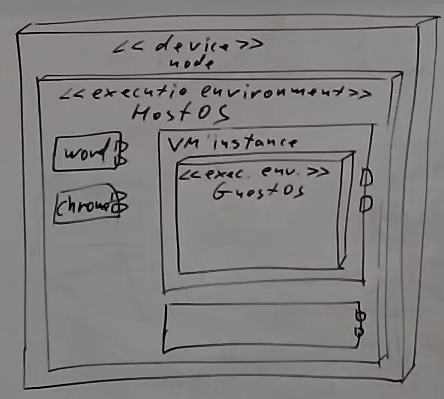
\includegraphics[width=0.7\linewidth]{Images/screenshot001}
        \end{figure}\noindent
        Объёмный параллелепипед~--- какой-то узел (физический, виртуальный или среда исполнения). Прямоугольник с двумя маленькими квадратиками~--- приложение.\\
        Одной программой живёт менеджер виртуальных машин. У него есть VM manager~--- ПО для управления виртуалками и при запуске появляется инстанс виртуальной машины как отдельное приложение. А там внутри эмулируется гостевая ОС, где внутри работают какие-то приложения.\\
        Ну, потому что что такое исполнение кода под ОС? Это отправка инструкций на процессор. Если они поддерживаются процессором и платформой, можно пробросить страницу с кодом в хостовую VM, и там исполнить. А если нет, то специальным алгоритмом одни команды подменяются на другие, чтобы работало.\\
        Это не просто, вообще написание эмуляторов~--- недёшево, но со временем менеджеры учились и сами запускаться много где и запускать много чего, поэтому VirtualBox сейчас запускает почти всё почти на всём. Но в чём проблема? В том что гостевая ОС ничего не знает про хост. А значит всё управление памятью у неё своё. Но никакого TLB-кэша нет, потому что с точки зрения хоста это всё одно приложение. А ещё у нас есть двойное вычисление адресов, что долго. То же верно для работы с железом. Гостевая ОС думает, что у неё есть сетевая плата, туда можно отправлять данные, и уже VM manager решает, что с этим делать (отправить на сетевую плату хоста).\\
        В итоге для домашнего использования ок, но работает капец медленно.
        \item Полная виртуализация.
        \begin{figure}[H]
            \centering
            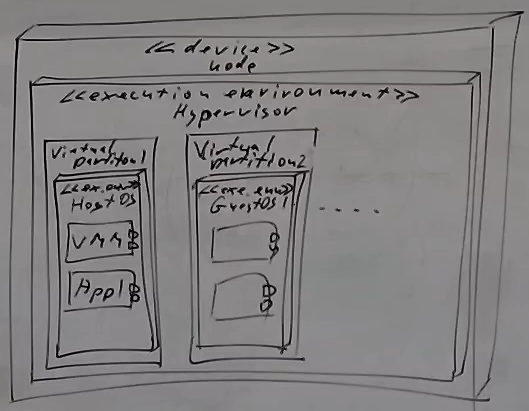
\includegraphics[width=0.7\linewidth]{Images/screenshot002}
        \end{figure}\noindent
        У нас есть гипервизор (система с наноядерной архитектурой), а дальше внутри его есть виртуальные партиции. Гипервизор умеет делать только несколько простых вещей: процессорное время она распределяет round-robin'ом (максимум можно настраивать разные кванты для разных виртуальных машин). А вот памятью гипервизор управляет хитро. Тут используются фиксированные разделы, каждый из который выделяется отдельной VM. И адреса фиксированы. Тогда все адреса можно пересчитывать очень легко, и никакой проблемы с каскадным вычислением адресов нет.\\
        Но тут вот какая проблема возникает: мы не научились решать проблему с работой с железом. Гипервизору мы не можем дать все драйвера (он больше не будет наноядерным). А делается там следующее: есть хостовая ОС, в которой есть драйвера. И есть два варианта:
        \begin{enumerate}
            \item Партиция никак не знает, что она виртуализирована. Тогда гипервизор перехватывает обращение и даёт их хостовой ОС.
            \item Второй вариант~--- гостевые дополнения (они же средства интеграции). Это драйвера, которые мы ставим гостевой ОС, чтобы она сама делала правильный вызов в гипервизор, чтобы он ничего не перехватывал и не преобразовывал. Это гипервызовом называется. Но такой драйвер ещё написать надо, а возможность это сделать есть не всегда.
        \end{enumerate}
        \item Но есть третий вариант: сделать в гостевой и хостовой ОС новый программный компонент: VM bus. В гостевой ОС это часть ядра, которая заставляет гостевую ОС не обращаться к драйверу, а кидает сообщение на шину, пока хостовая ОС слушает эту шину. Это быстро, но работает только если ядро можно модифицировать. Такое (когда мы разворачиваем ОС с модифицированным ядром) называется \textbf{паравиртуализация}.
        \item Окей, есть 100500 гостевых Linux'ов. Но блин, у них всех одно ядро, зачем его дублировать в памяти? Идея такая: внутри нашей ОС сделаем контейнер как группу процессов.
        \begin{figure}[H]
            \centering
            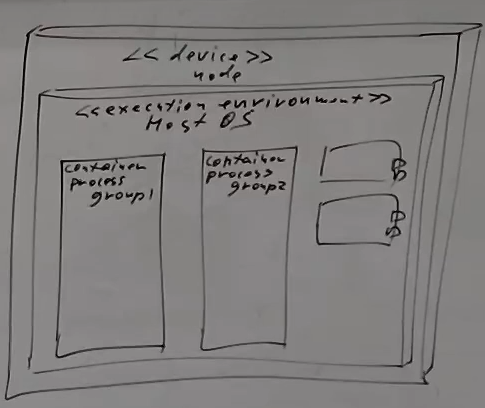
\includegraphics[width=0.7\linewidth]{Images/screenshot003}
        \end{figure}\noindent
        Помните, что у нас были контрольные группы (возможность поставить квоту на использование ресурсов для группы процессов)? И помните процесс с PID'ом 1? На самом деле он также обеспечивает доставку сигналов. Так вот каждый контейнер имеет свой собственный init/systemd, и это обеспечивает неплохую изоляцию, но при этом обеспечиваем использование только одного ядра. Эффективно по времени и памяти.\\
        Минусы также очевидны~--- все приложения гостевой ОС должны быть совместимы с хостовой. Второе~--- таблица процессов никуда не девается. Если в одном контейнере плодятся зомби, у нас и хостовая ОС умрёт
    \end{enumerate}
    \paragraph{Классификация по типу виртуализируемой среды.}
    \begin{enumerate}
        \item Виртуализация представлений~--- не виртуализируются ресурсы, процессы, а только их представление пользователю. Простой пример~--- сервер терминалов Windows. 
        \item Виртуализация рабочих мест~--- с точки зрения пользователя операционная система со всем ПО где-то удалена.
        \item Виртуализация серверов~--- как виртуализация рабочих мест, но без GUI.
        \item Виртуализация приложений~--- когда без установки и развертывания ПО запускаете приложение. Вроде как приложению нужно быть интегрированным в ОС. А тут берётся очень урезанная среда виртуализации, туда ставится крайне урезанная версия ОС, и туда ставится приложение. Понятно, что это безнадёжно тормозит.
    \end{enumerate}
    \paragraph{Облако.}
    А дальше людям пришло в голову, что можно узлы с виртуальными машинами объединить в одну систему. И получилась вот какая модель.
    \begin{figure}[H]
        \centering
        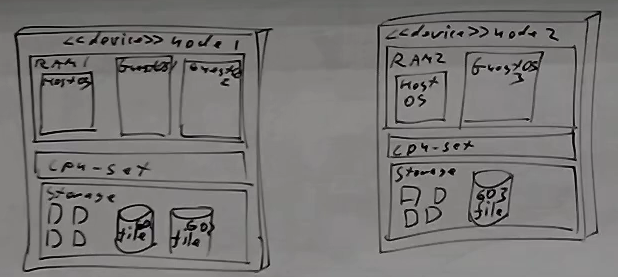
\includegraphics[width=0.7\linewidth]{Images/screenshot004}
    \end{figure}\noindent
    Для хостовой ОС у нас какие-то файлики, а все файлы гостевых ОС~--- один большой файл.\\
    Теперь представим, что гостевые ОСи 1 и 2 потеют и выжирают весь процессор, а гостевая ОС 3 чиллит. Может имеет смысл перенести гостевую ОС 2 в другую хостовую ОС? Смотрите, у нас была задача переносить задачу, и мы всю прошлую лекцию страдали, думая, как же перенести процесс. А мы хотим перенести сразу виртуальную операционную систему. В чём проблема? В том, что в гостевой ОС есть не только оперативка (которой не очень много), но и хранилище, которого может быть под терабайт, и его уже фиг перекачаешь.\\
    Но тут на помощи пришли
    \subparagraph{Физические системы хранения данных.}
    Это компьютер со специализированной ОС, который умеет только хранить данные. Зато как хорошо: там не то что RAID 5, там есть диски быстрые, диски медленные, какие-то совершенно нетривиальные взаимодействия, сжатие пр передаче, кэши и всё-всё-всё. Для пользователя это представлено так называемыми LUN'ами~--- logical unit. И дальше мы каждый файл каждой гостевой ОС помещаем в свой LUN.
    \begin{figure}[H]
        \centering
        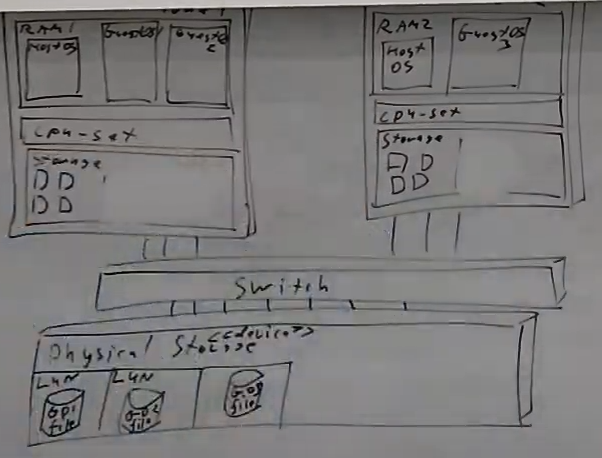
\includegraphics[width=0.7\linewidth]{Images/screenshot005}
    \end{figure}\noindent
    Осталось только смонтировать файловую систему как сетевую файловую систему. И всё у нас хорошо.\\
    Но всё не так просто. Мы откуда-то знали, что на одном узле всё хорошо, а на другом~--- плохо. Надо как-то узнавать, что на каком узле плохо. В простых системах можно использовать polling~--- опрашивать каждый узел равные промежутки времени. Чем чаще его делать, тем сильнее нагружаются ресурсы, но тем менее актуальная у нас информация.\\
    Второй вариант~--- интеллектуальные агенты. В каждую хостовую ОС посадим демона, который при запуске будет говорить специальному выделенному узлу, что такая хостовая ОС есть. А демону в ответ приходят пороги срабатывания: если будет пало памяти в течение некоторого времени или ещё чего, он будет спрашивать у этого выделенного узла, что делать? И тот будет решать, это всем плохо (и надо повысить пороги) или над перенести.\\
    Но как решать, кого и куда перенести? Как быть уверенным, что миграция гостевой ОС нам поможет? (А миграция~--- не очень дёшево, если что, у нас просаживается сеть, просаживается производительность и узла, откуда мигрируют, и узла, куда). Причём мигрировать не только виртуалку, но и контейнер, например. И тут уже недо для каждой конкретной ситуации решать свою задачу и страдать.\\
    Но это ладно, давайте обсудим ещё, что в современных облаках есть ещё одна интересная концепция: шаблоны. В физической системе хранения данных создаются уже настроенные файлики для разных задач: если вы хотите развернуть СУБД, вам тупо дают готовую.
\end{document}
